\documentclass{article}
\usepackage[utf8]{inputenc}
\usepackage{indentfirst}
\usepackage{titling}
\usepackage{geometry}
\usepackage{graphicx}
\graphicspath{ {./Images/} }
\usepackage[shortlabels]{enumitem}
\usepackage{fancyhdr}
\usepackage{ulem}
\usepackage[dvipsnames]{xcolor}
\usepackage{amssymb}
\usepackage{listings}
\usepackage{color}

\definecolor{dkgreen}{rgb}{0,0.6,0}
\definecolor{gray}{rgb}{0.5,0.5,0.5}
\definecolor{mauve}{rgb}{0.58,0,0.82}

\lstset{frame=tb,
  language=Java,
  aboveskip=3mm,
  belowskip=3mm,
  showstringspaces=false,
  columns=flexible,
  basicstyle={\small\ttfamily},
  numbers=none,
  numberstyle=\tiny\color{gray},
  keywordstyle=\color{blue},
  commentstyle=\color{dkgreen},
  stringstyle=\color{mauve},
  breaklines=true,
  breakatwhitespace=true,
  tabsize=3
}

\def\ojoin{\setbox0=\hbox{$\bowtie$}%
  \rule[-.02ex]{.25em}{.4pt}\llap{\rule[\ht0]{.25em}{.4pt}}}
\def\leftouterjoin{\mathbin{\ojoin\mkern-5.8mu\bowtie}}
\def\rightouterjoin{\mathbin{\bowtie\mkern-5.8mu\ojoin}}
\def\fullouterjoin{\mathbin{\ojoin\mkern-5.8mu\bowtie\mkern-5.8mu\ojoin}}

\renewcommand\maketitlehooka{\null\mbox{}\vfill} %para centralizar verticalmente
\renewcommand\maketitlehookd{\vfill\null}
\pagestyle{fancy}
\fancyhf{}
\rfoot{\thepage}
\lfoot{ 
\includegraphics[scale=0.01]{UA.jpg} José Mendes 107188 LEI}
\geometry{
  a4paper,
  headheight=4cm,
  top=5.5cm,
  bottom=4.5cm,
  footskip=4cm
}


\title{Introdução à Engenharia de Software}
\author{José Mendes 107188}
\date{2023/2024}

\begin{document}


\begin{titlepage}
    \maketitle
    \begin{center}
        
\includegraphics[scale=0.4]{UA.png}
    \end{center}
    \thispagestyle{empty} %remove o count da pagina
\end{titlepage}

\pagebreak

\section{Maven}

\subsection{O que é o Maven?}

É uma \textbf{ferramenta de gestão de projetos}, que inclui:
\begin{itemize}
  \item Um \textbf{project object model} (POM) que descreve o projeto;
  \item Um conjunto de \textbf{standards};
  \item Um \textbf{lifecycle} do projeto;
  \item Um sistema de gestão de \textbf{dependências};
  \item Lógica para \textbf{executar plugins} em \textbf{fases} específicas
  do ciclo de vida.
\end{itemize}

Convenção sobre configuração (layout do projeto é padronizado).

\subsection{Layout de Diretórios Padronizado}

\begin{flushleft}
  \textbf{POM} - Contém uma descrição completa do projeto de como
  construir o projeto.

  \vspace{2mm}

  \textbf{src} - Diretório que contém todo o código fonte para construir
  o projeto, o seu site, \dots

  \vspace{2mm}

  \textbf{target} - Diretório que contém os resultados da construção,
  tipicamente um JAR ou WAR, juntamente com os ficheiros intermedios.
\end{flushleft}

\subsection{POM}

Maven é baseado no conceito de um \textbf{Project Object Model} (POM).
Este é um ficheiro XML, que está sempre localizado no diretório base do projeto
como \textbf{pom.xml} (os users definiram POMs que estendem o Super POM).

O POM contém informação sobre o projeto e vários detalhes de configuração
usados pelo Maven para construir o projeto.

O POM é declarativo, não necessita de detalhes de procedimento.

\subsubsection{Estrutura do POM}

\begin{flushleft}
  O POM contém 4 categorias de descrição e configuração:
  
  \begin{itemize}
    \item Informação geral do projeto, isto é, informação human-readable;
    \item Configuração do build, que pode incluir, adicionar plugins,
    afixar plugins objetivo ao ciclo de vida;
    \item Ambiente de construção, que descreve o ambiente "familiar" em que o Maven está;
    \item Relações POM, isto é, coordenadas, herança, agregação, dependências.
  \end{itemize}
\end{flushleft}

\pagebreak

\subsection{Coordenadas Maven}

As coordenadas definem o lugar único do projeto no universo Maven.
São compostas por 3 partes: \textbf{$<$groupId$>$}, \textbf{$<$artifactId$>$} e
\textbf{$<$version$>$} (The Maven trinity!).

\vspace{2mm}

As versões de um projeto são usadas para agrupar e ordenar lançamentos:

\[ <major\_version>.<minor\_version>.<incremental\_version>-<qualifier> \]

\begin{flushleft}
  \textbf{Exemplo:} 1.0.0-SNAPSHOT ou 1.2.3-alpha-2
\end{flushleft}

Se o qualifier contiver a palavra chave SNAPSHOT, então o Maven
vai expandir este token para uma data e hora convertida para o formato UTC.

\vspace{2mm}

\begin{flushleft}
  \begin{itemize}
    \item \textbf{groupId} - Nome da empresa, organização, equipa, \dots,
    normalmente usando a convenção de nomes de domínio invertidos (reverse URL naming, ex: org.apache.maven);

    \item \textbf{artifactId} - Nome único do projeto dentro do groupId;
    
    \item \textbf{version} - Versão do projeto;
    \item \textbf{packaging} - Tipo de empacotamento do projeto (jar (default), war, \dots);
    \item \textbf{classifier} - Classificador opcional para distinguir artefactos
  \end{itemize}

  \vspace{2mm}

  \textbf{Nota:} As coordenadas Maven identificam unicamente um projeto.
\end{flushleft}

\subsection{Ciclo de Vida Maven}

Um ciclo de vida é uma sequência organizada de fases,
que dão ordem a uma sequência de objetivos.
Estes objetivos são empacotados em plugins que estão ligados
as fases.

\begin{center}
  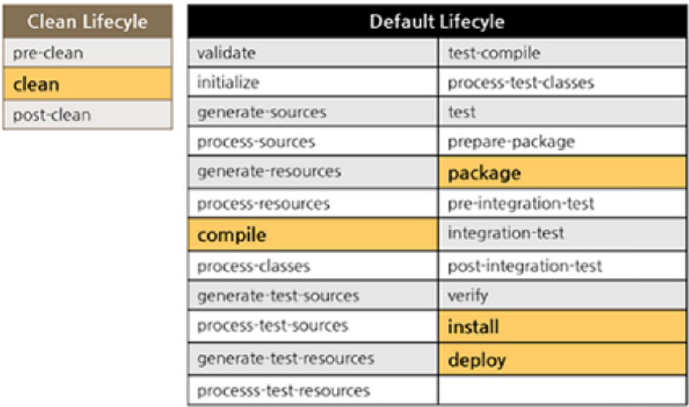
\includegraphics[scale=0.5]{1}
\end{center}

Chamar uma fase específica num ciclo de construção, vai executar
todas as fases anteriores a essa fase.

\pagebreak

\begin{center}
  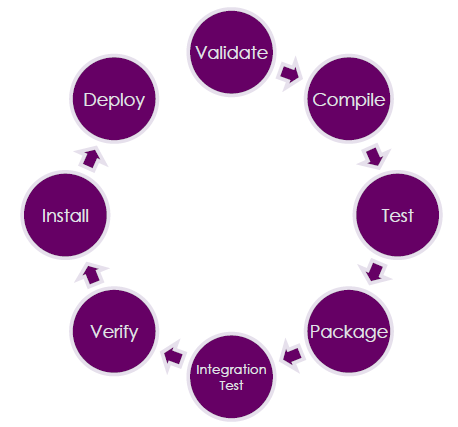
\includegraphics[scale=0.5]{2}
\end{center}

\begin{flushleft}
  \begin{enumerate}
    \item \textbf{Validate} - Valida que a estrutura do projeto está correta.
    (ex: verifica se todas as dependências foram transferidas e estão disponíveis
    no repositório local);

    \item \textbf{Compile} - Compila o código fonte, converte os ficheiros
    \textbf{.java} em \textbf{.class}, e armazenando-os no diretório \textbf{target/classes};

    \item \textbf{Test} - Corre testes unitários para o projeto;
    \item \textbf{Package} - Empacota o código compilado num formato distribuível
    como \textbf{JAR} ou \textbf{WAR};

    \item \textbf{Integration Test} - Corre testes de integração para o projeto;
    \item \textbf{Verify} - Corre verificações para verificar que o projeto é válido
    e que cumpre os critérios de qualidade;

    \item \textbf{Install} - Instala o código empacotado
    no repositório Maven local, para uso como dependência noutros projetos locais;

    \item \textbf{Deploy} - Copia o pacote final de código para o repositório
    remoto para partilha com outros developers e projetos.
  \end{enumerate}
\end{flushleft}

\subsection{Ciclo de Vida de Construção}

O processo para contruir e distribuir um projeto. Consiste
em vários passos designados por \textbf{fases}.

Algumas fases default são:
\begin{itemize}
  \item \textbf{validate}
  \item \textbf{compile}
  \item \textbf{test}
  \item \textbf{package}
  \item \textbf{deploy}
\end{itemize}

\pagebreak

\subsection{Goals e Plugins}

Os Goals são operações fornecidas pelas ferramentas Maven.

Cada fase é uma sequência de Goals, em que cada Goal é responsável
por uma tarefa específica. Quando corremos uma fase, todos os Goals
ligados a essa fase são executados, na ordem em que estão definidos.

\begin{flushleft}
  Algumas Maven Plugins:
  \begin{itemize}
    \item resources
    \item compiler
    \item surefire
    \item jar, war
  \end{itemize}
\end{flushleft}

\subsection{Arquétipos (Archetypes)}

Um Archetype é um template para um projeto Maven, que pode ser usado para
criar um novo projeto rapidamente.

\begin{flushleft}
  \textbf{Exemplo:} \textit{maven-archetype-quickstart} ou \textit{maven-archetype-webapp}
\end{flushleft}

Users podem criar os seus próprios Archetypes e publicá-los através de catálogos.

\subsection{Gestor de Dependências}

Uma \textbf{dependência} de um projeto é uma biblioteca da qual
o projeto depende. Adicionar uma dependência ao projeto é simples,
basta adicionar a dependência ao POM. O Maven vai automaticamente
procurar a dependência no repositório local, e se não encontrar,
vai procurar no repositório remoto e transferi-la.

\begin{center}
  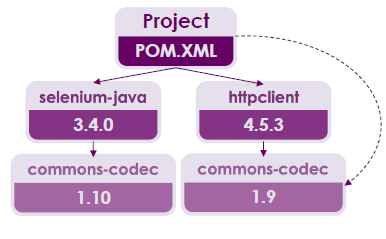
\includegraphics[scale=0.6]{3}
\end{center}

\pagebreak

\section{Git e GitHub}

\subsection{Sistemas de Controlo de Versões}

Um sistema de controlo de versões (também conhecido como sistema de controlo de código fonte) faz o seguinte:
\begin{itemize}
  \item Mantém várias (antigas e novas) versões de tudo (não só código fonte);
  \item Pede por comentários quando se fazem alterações;
  \item Permite "check-in" e "check-out" de ficheiros para saber
  em que ficheiros outras pessoas estão a trabalhar;
  \item Mostra as diferenças entre versões;
\end{itemize}

\subsubsection{Vantagens}

\begin{flushleft}
  \textbf{Ao trabalhar sozinho:} Fornece uma "máquina do tempo" para
  voltar atrás para uma versão anterior, e fornece um bom suporte 
  de diferentes versões do mesmo projeto.

  \vspace{2mm}

  \textbf{Ao trabalhar em equipa:} Simplifica muito trabalhar em concurrencia,
  dando "merge" de alterações feitas por diferentes pessoas.
\end{flushleft}

\subsection{o que é Git e GitHub}

\begin{center}
  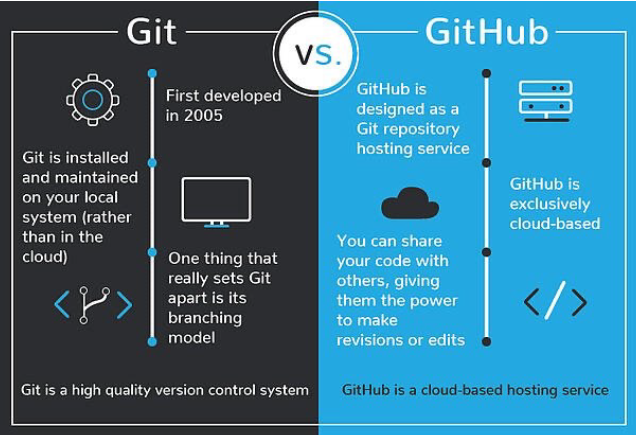
\includegraphics[scale=0.5]{4}
\end{center}

Quando fazemos "git init" num diretório de um projeto, ou quando fazemos
"git clone" de um projeto existente, o Git cria um repositório (.git).

Em qualquer momento, podemos fazer um "snapshot" de tudo
no dirétorio do projeto e guardar este no repositório.
Este "snapshot" é chamado de \textbf{commit object}.

\pagebreak

Um \textbf{commit} ocorre quando fazemos alterações que estão
prontas para serem guardadas no repositório.

Quando realizamos um commit, o Git guarda um \textbf{commit object}:
\begin{itemize}
  \item Um estado completo do projeto, incluindo todos os ficheiros;
  \item O primeio não possui pai;
  \item Normalmente, pegamos num commit object, fazemos alterações,
  e criamos um novo commit object, pelo que a maior parte dos commit objects
  têm apenas um pai;
  \item Quando fazemos \textbf{merge} de dois commit objects,
  forma um commit object com dois pais.
\end{itemize}

Pelo que, os commit objects formam uma \textbf{DAG} (Directed Acyclic Graph).
O Git é tudo sobre usar e manipular este grafo.

\subsubsection{Mensagem de Commit}

Os commits são "baratos" pelo que os devemos fazer com frequência, e com
mensagens descritivas sobre o que foi alterado. Devem ter apenas uma linha.

Como não devemos dizer muito numa linha, devemos fazer vários commits.

\begin{center}
  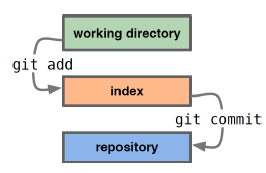
\includegraphics[scale=0.6]{5}
\end{center}

\subsection{Manter simples}

\begin{center}
  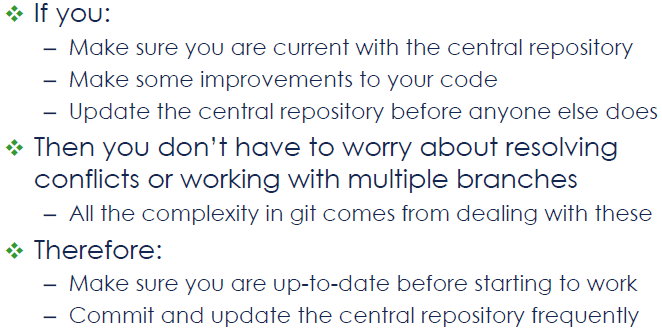
\includegraphics[scale=0.6]{6}
  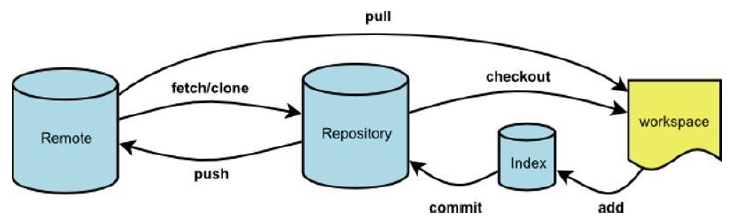
\includegraphics[scale=0.6]{7}
\end{center}

\pagebreak

\section{O Processo de Desenvolvimento de Software}

\subsection{Processo}

A fundação para a Engenharia de Software é a camada de processo.
Um processo de Software é uma framework para as atividades,
ações, e tarefas necessárias para construir software de alta qualidade.
Define as técnicas e a framework de gestão para aplicação de métodos,
ferramentas e pessoas ao longo do processo de desenvolvimento.

\begin{center}
  
\includegraphics[scale=0.6]{8}
\end{center}

\subsection{Porquê o Processo de Software?}

\begin{center}
  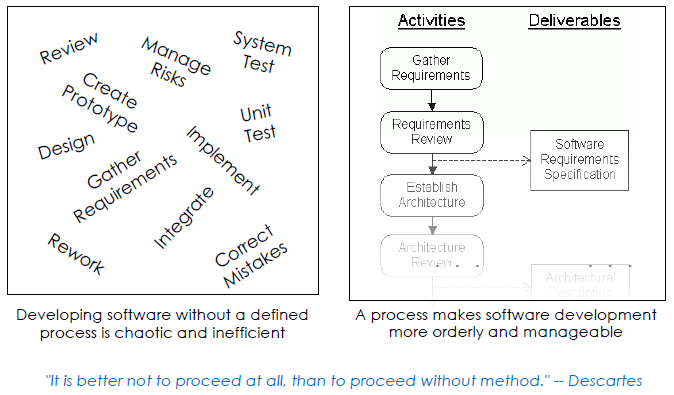
\includegraphics[scale=0.6]{9}
\end{center}

\subsection{Processo de Software}

Existem vários tipos de processos de software, no entanto, todos têm:

\begin{itemize}
  \item \textbf{Especificação (comunicação e planeamento)} - definir o que o sistema deve fazer;
  \item \textbf{Design e Implementação} - definir a organização do sistema e implementar o sistema;
  \item \textbf{Validação} - verificar que faz aquilo que o cliente quer;
  \item \textbf{Evolução} - alterar o sistema em resposta a novos requisitos impostos pelo cliente.
\end{itemize}


Quando discutimos sobre o processo de software, estamos a falar sobre:
\begin{itemize}
  \item \textbf{Atividades} - como especificar um modelo de dados, design de uma
  interface de utilizador, \dots;
  \item \textbf{Ordem} a ordem destas atividades;
\end{itemize}

A descrição de processos pode também incluir, \textbf{produtos} (outcome da
atividade do processo), \textbf{papéis} (roles, responsabilidades das pessoas envolvidas)
e \textbf{pré-/pós-condições} (são condições que são verdadeiras antes
e depois de atividade do processo ou de um produto ser produzido).

\pagebreak

O processo de software específica:
\begin{itemize}
  \item \textbf{O quê}
  \item \textbf{Quem}
  \item \textbf{Quando}
  \item \textbf{Como}
\end{itemize}

E incluí
\begin{itemize}
  \item \textbf{Papéis} (Roles)
  \item \textbf{Fluxo de trabalho} (Workflow)
  \item \textbf{Procedimentos} (Procedures)
  \item \textbf{Normas} (Standards)
  \item \textbf{Modelos} (Templates)
\end{itemize}

\subsection{Pontos Chave}

\textbf{\uline{O processo de Software é um guia}}

\vspace{2mm}

Não existe "um melhor processo para escrever software".
Um processo que um individuo ou uma organização escolhe e segue depende de:
\begin{itemize}
  \item das características específicas do projeto;
  \item da cultura da organização;
  \item das habilidades e preferências das pessoas envolvidas.
\end{itemize}

\vspace{2mm}

Um bom processo aumenta a produtividade de membros da equipa
menos experientes sem impedir o trabalho/progresso de membros
mais experientes.

\subsection{Resistência ao Processo de Software}

\begin{flushleft}
  \textbf{Perceção:} Algumas pessoas vêm seguir um processo como
  uma sobrecarga (overhead) desnecessária na produtividade.
  \begin{itemize}
    \item Interfere com a criatividade;
    \item Burocracia e regimento;
    \item Prejudica a agilidade em mercados que evoluem rapidamente.
  \end{itemize}

  \vspace{2mm}

  \textbf{A realidade:} Grupos que não seguem um processo definido
  tendem a adicionar processo mais tarde no projeto, como reação
  a problemas que surgem. Quando o tamanho e a complexidade do projeto
  aumenta, a importância de seguir processos definidos aumenta proporcionalmente. 
\end{flushleft}

\pagebreak

\subsection{Fases de Software}

\begin{center}
  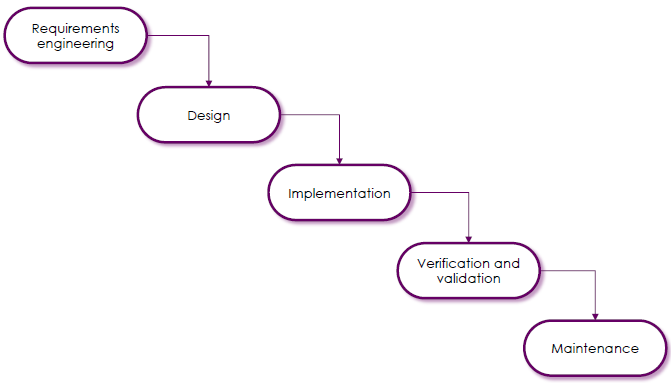
\includegraphics[scale=0.6]{10}
\end{center}

\subsection{\uline{Modelos} de Processo de Software}

Modelos abstratos que descrevem uma classe abordagens de desenvolvimento
com características similares.

\vspace{2mm}

Alguns critérios utilizados para distinguir modelos de processos
de software são:
\begin{itemize}
  \item o tempo entre fases (timing);
  \item critérios de entrada e saída entre fases (entry/exit criteria);
  \item os artefactos criados durante cada fase;
\end{itemize}

\vspace{2mm}

Alguns \textbf{exemplos} incluem: Waterfall, Spiral, Rapid Prototyping,
Incremental, Development, \dots

\subsubsection{Modelos (Tradicionais)}

\begin{flushleft}
  \textbf{Modelo em Cascata (Waterfall):} É um modelo \uline{Plan-Driven}.
  Separa e distingue fases de especificação e desenvolvimento.

  \vspace{2mm}

  \textbf{Desenvolvimento Incremental:} A especificação, desenvolvimento
  e validação são intercalados. Pode ser \uline{Plan-Driven} ou \uline{Agile}.

  \vspace{2mm}

  \textbf{Processos Evolucionários/Iterativos:} O sistema é desenvolvido
  no ínicio usando uma especificação muito simples, sendo modificada
  e melhorada de acordo com as necessidades de software.

  \vspace{2mm}

  \textbf{Muitos outros:} A maior parte de sistemas grandes são desenvolvidos
  usando um processo que incorpora elementos de diferentes modelos.
\end{flushleft}

\pagebreak

\subsubsection{O Modelo em Cascata (Waterfall)}

\begin{center}
  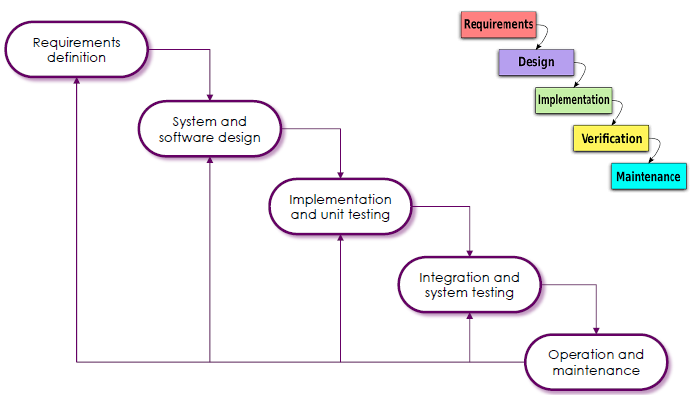
\includegraphics[scale=0.6]{11}
\end{center}

\subsubsection*{Vantagens}

\begin{itemize}
  \item É simples e fácil de perceber e usar;
  \item É fácil de planear, um schedule pode ser definido
  com deadlines para cada fase de desenvolvido e um produto pode ser
  processado através do processo de desenvolvimento como um carro
  numa lavagem automática, e ,teoricamente, ser entregue a tempo.
  \item Fácil de gerir, cada fase tem entregas específicas e um
  processo de revisão.
  \item Fases e processos são concluídos um de cada vez.
  \item Funciona bem onde os requisitos são bem compreendidos.
\end{itemize}

\subsubsection*{Desvantagens}

\begin{itemize}
  \item Dificuldade em acomodar mudanças após o processo começar.
  Em principio, uma fase deve ser concluída antes de começar a próxima.
  Particionamento inflexível do projeto em fases distintas torna difícil
  responder a mudanças nos requisitos do cliente.
  \item Modelo não muito bom para projetos de longa duração ou que já estão em andamento
  (não é produzido nenhum software funcional até mais tarde no ciclo de vida).
  \item Não é adequado a processos onde os requisitos são incertos ou
  onde há risco de serem alterados.
\end{itemize}

\pagebreak

\subsubsection{Modelo Incremental}

Uma característica de modelos com ciclos de vida modernos.
O produto evolui através de uma série de iterações.

\begin{center}
  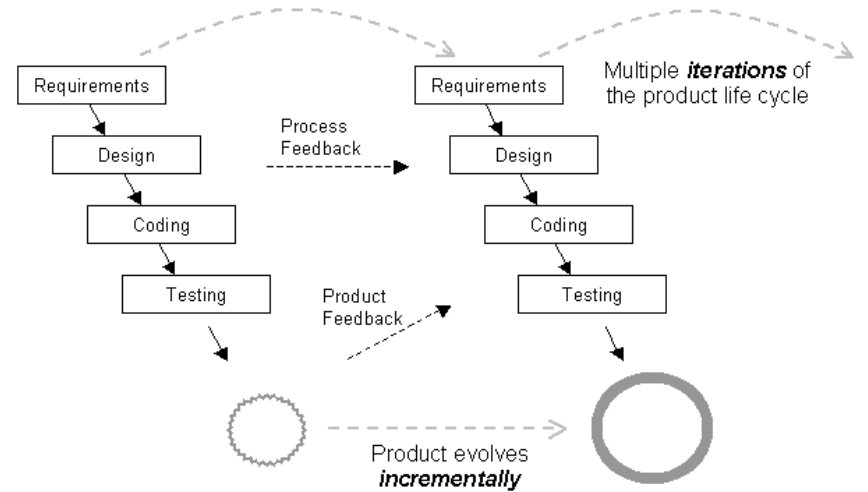
\includegraphics[scale=0.5]{12}
\end{center}

\subsubsection*{Benefícios}

\begin{itemize}
  \item O custo de \textbf{acomodar mudanças de requisitos do cliente} é reduzido.
  A quantidade de análise e documentação que tem de ser refeita é muito menor
  do que no modelo em cascata.

  \item É mais fácil \textbf{obter feedback do cliente} sobre o desenvolvimento
  do trabalho que já está concluído.
  Clientes podem comentar sobre demonstrações do software e ver
  quanto foi implementado.

  \item \textbf{Entrega mais rápida e deployment} do software útil
  para o cliente é possível. Os clientes podem usar e ganhar valor
  do software mais cedo do que se o sistema fosse desenvolvido
  com o processo em cascata.
\end{itemize}

\subsubsection*{Problemas}

\begin{itemize}
  \item \textbf{Cada fase de iteração é rigida} e não se sobrepoem
  umas com as outras.

  \item O processo não é visível. Os gestores precisam  de entragas regulares
  para medir o progresso. No entanto, se o sistema não for desenvolvido rapidamente,
  não é cost-effective produzir documentos que reflitam cada versão do sistema.

  \item A estrutura do sistema tende a degradar-se à medida que novos
  incrementos são adicionados. A não ser que tempo e dinheiro seja
  gasto na refatoração para melhorar o software,
  \textbf{regular mudanças tende a corromper a sua estrutura}.
  A medida que vamos incorporando novas mudanças de doftware,
  torna-se mais difícil e mais caro.
\end{itemize}

\pagebreak

\subsubsection{Modelos Evolucionários/Iterativos}

\begin{flushleft}
  \textbf{Prototipagem:} Geralmente, um cliente define um conjunto
  de objetivos gerais para o software, mas não identifica requisitos
  detalhados para funções e funcionalidades do sistema.

  \vspace{2mm}

  \textbf{Modelo Espiral:} Utilizando um modelo espiral, o software é desenvolvido
  numa serie de lançamentos (releases) evolutivos. Durante as primeiras iterações,
  o lançamento pode ser um protótipo ou um modelo.

  \vspace{2mm}

  \textbf{Modelo Concurrente:} Permite a uma equipa de software representar
  elementos iterativos e concurrentes de quaisquer modelos de processo.
\end{flushleft}

\subsubsection{Incremental vs Evolucionário/Iterativo}

\begin{center}
  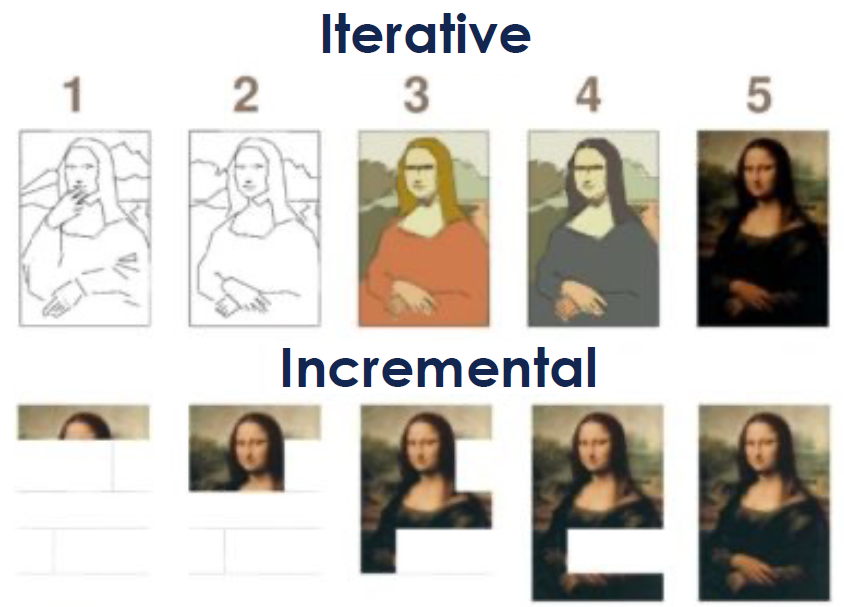
\includegraphics[scale=0.5]{13}
\end{center}

\subsubsection{Exemplos}

\begin{center}
  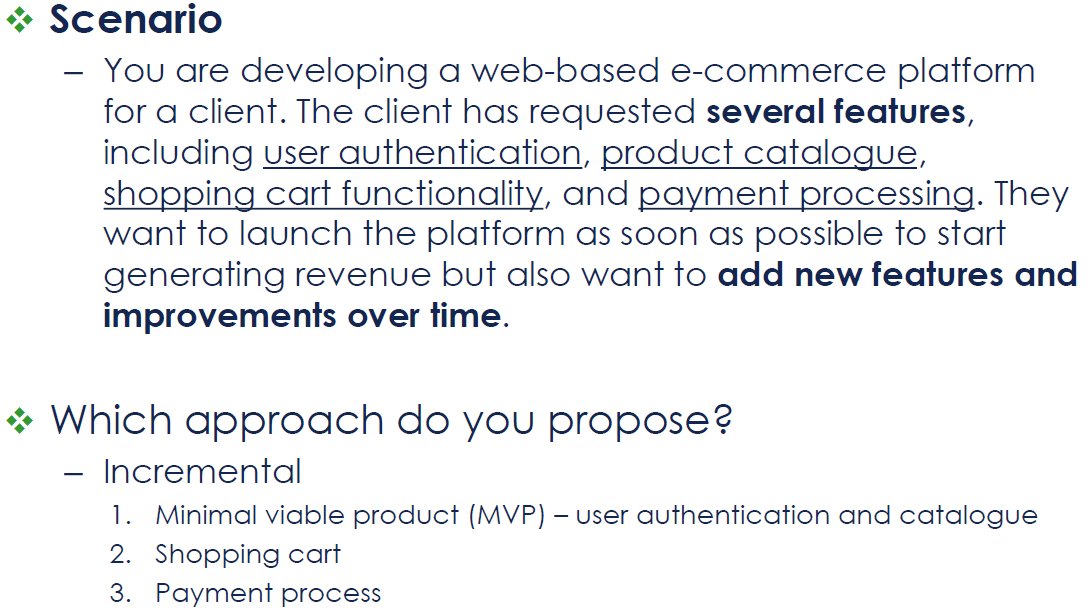
\includegraphics[scale=0.32]{14}
  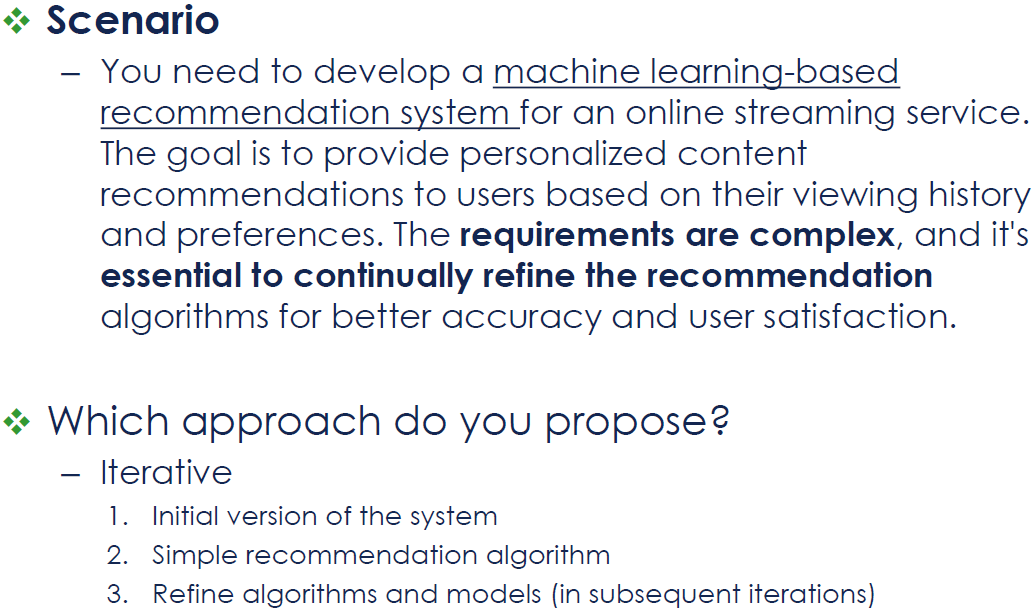
\includegraphics[scale=0.32]{15}
\end{center}

\pagebreak

\subsection{Outros Modelos de Processo}

\begin{itemize}
  \item Desenvolvimento \textbf{Component-Based} (COTS): O processo
  para aplicar quando reutilizar é um objetivo do desenvolvimento.

  \item \textbf{Métodos Formais}: Enfatiza a especificação matemática
  dos requisitos.

  \item \textbf{Processo Unificado (UP)}: Um processo de software
  "use-case driven, arquitetura-centric, iterativo e incremental",
  alinhado com o Unified Modeling Language (UML).
\end{itemize}

\subsection{Processo Unificado (UP)}

\begin{center}
  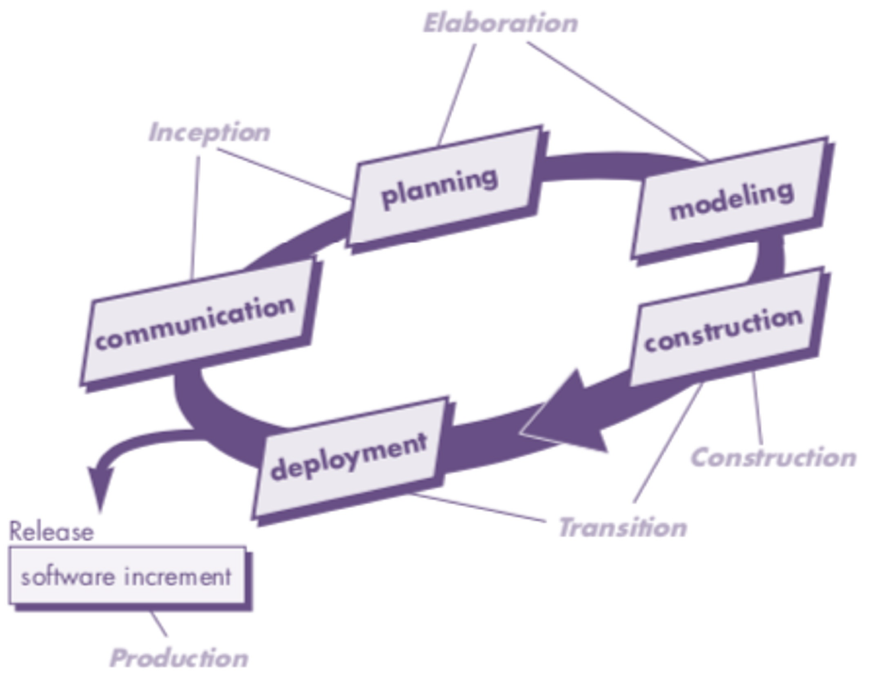
\includegraphics[scale=0.4]{16}
\end{center}

\subsubsection{Fases}

\begin{center}
  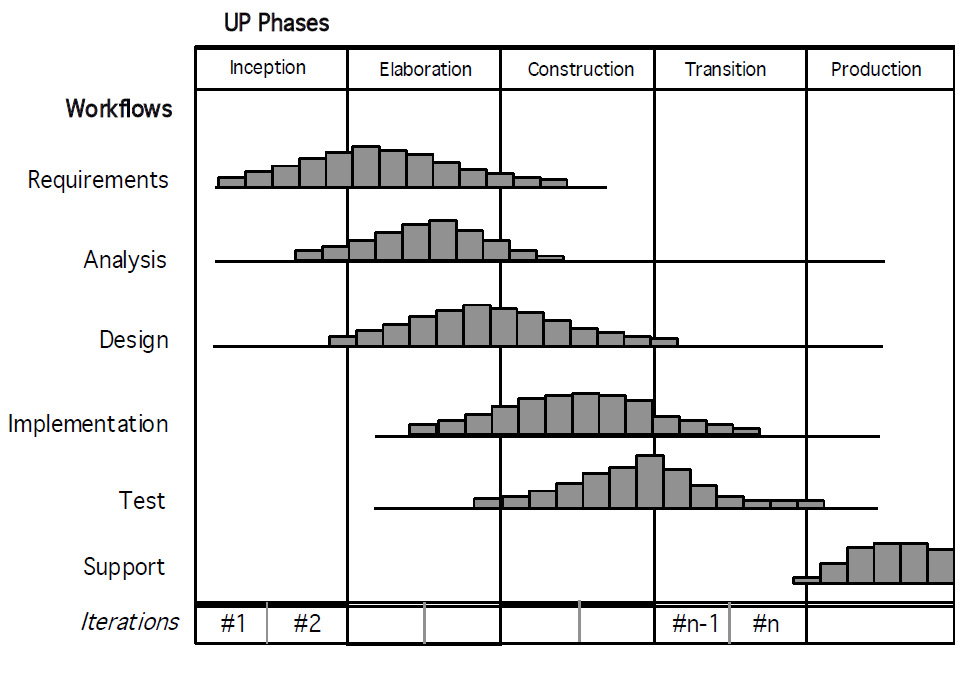
\includegraphics[scale=0.4]{17}
\end{center}

\pagebreak

\subsection{Processos Plan-Driven e Agile}

\textbf{Processos Plan-Driven} são processos onde todas as atividades
são planeadas \uline{anteciadamente} e o progresso é medido
contra este plano.

\vspace{2mm}

Em \textbf{Processos Agile}, planear é incremental e é mais fácil
mudar o processo para refletir a mudança nos requisitos do cliente.

\vspace{2mm}

Na prática, a maior parte dos processos incluem elementos de ambos,
processos plan-driven e agile. Não existem processos de software
"certos" ou "errados".

\subsubsection{Processos Plan-Driven vs Agile}

\begin{center}
  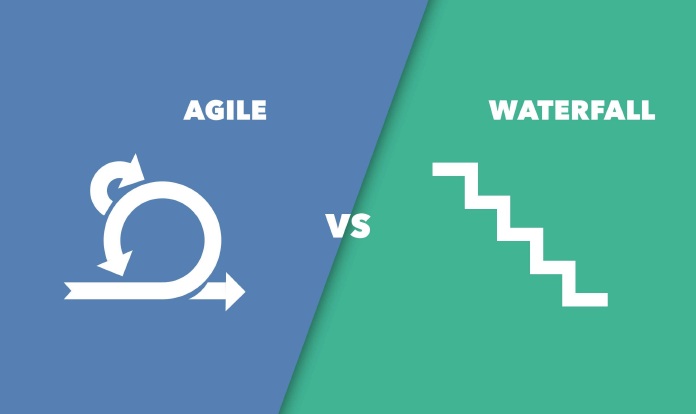
\includegraphics[scale=0.5]{18}
\end{center}

\subsubsection{Processos Agile}

Desenvolvimento rápido e entragas são, geralmente, os requisitos
mais importantes para sistemas de software.
\begin{itemize}
  \item Negócios operam num ambiente \textbf{fast-changing requirements}
  e é praticamente impossível produzir um conjunto de requisitos de software
  estáveis.
  \item O Software deve evoluir rapidamente para refletir mudanças de
  negócios.
\end{itemize}

\vspace{2mm}

Desenvolvimento Plan-Driven é essencialmente para alguns tipos de sistemas
mas não cobre as necessidades do negócio.

\subsubsection*{Métodos Agile}

\begin{itemize}
  \item Métodos Agile foram desenvolvidos num esforço para ultrapassar
  fraquezas percetidas e reais em engenharia de software convencional.
  
  \item \textbf{Foca no código em vez de no design}.
  
  \item Baseados em \textbf{abordagens iterativas} ao desenvolvimento
  de software.

  \item Tem a intenção de \textbf{entregar software funcional rapidamente}
  e evoluir rapidamente para refletir mudanças de requisitos do cliente.
\end{itemize}

\pagebreak

\subsubsection{Origem: Manifesto Agile}

"We are uncovering better ways of developing
software by doing it and helping others do it.
Through this work we have come to value:

\begin{itemize}
  \item \textbf{Individuals and interactions} over processes and tools
  \item \textbf{Working software} over comprehensive documentation
  \item \textbf{Customer collaboration} over contract negotiation
  \item \textbf{Responding to change} over following a plan
\end{itemize}

That is, while there is value in the items on the right,
we value the items on the left more."

\subsubsection{Princípios dos Métodos Agile}

\begin{flushleft}
  \textbf{Involvimento do cliente:} Os clientes devem estar envolvidos
  durante todo o porcesso de desenvolvimento. O seu papel é fornecer
  e priorizar novos requisitos e avaliar as iterações do sistema.
\end{flushleft}

\subsubsection{Desenvolvimento Plan-Driven e Agile}

\begin{center}
  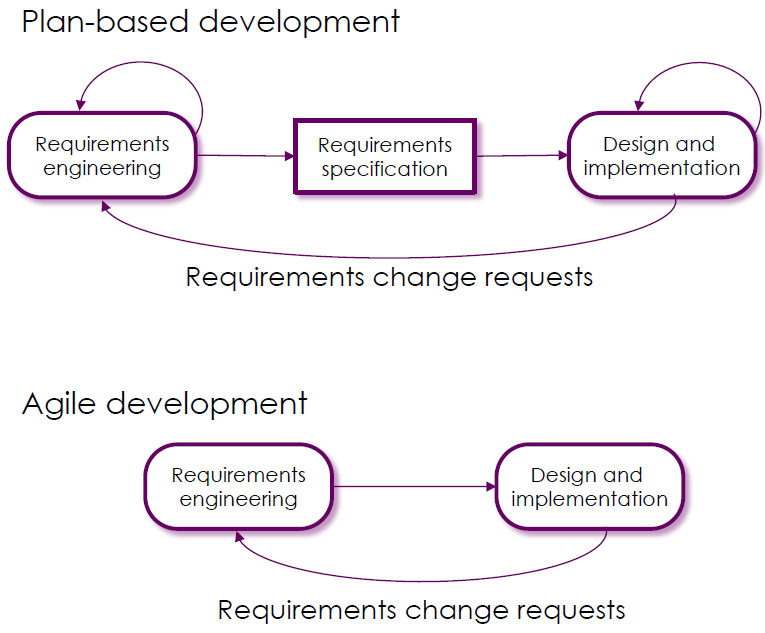
\includegraphics[scale=0.4]{19}
\end{center}

\begin{flushleft}
  \textbf{Desenvolvimento Plan-Driven:}
  \begin{itemize}
    \item Baseado ao redor de um desenvolvimento separado de fases,
    com outputs a serem produzidos em cada fase planeada anteciadamente.
    \item Não é necessariamente o modelo em cascata - desenvolvimento
    incremental, plan-driven, é possível.
  \end{itemize}

  \vspace{2mm}

  \textbf{Desenvolvimento Agile:}
  \begin{itemize}
    \item Especificação, design, implementação e testes são intercalados.
    \item Os outputs do processo de desenvolvimento são decididos
    através de um processo de negociação durante o processo de desenvolvimento
    de software.
  \end{itemize}
\end{flushleft}

\pagebreak

\subsubsection{Métodos Agile - Benefícios}

\begin{itemize}
  \item Requisitos num modelo Agile podem ser alterados
  conforme os requisitos do cliente mudam. Por vezes os requisitos
  não são muito claros. Mudanças nos requisitos são aceites
  mesmo em fases avançadas do processo de desenvolvimento.

  \item A entrega de software é continua. Clientes podem seguir
  cada feature funcional do Sprint do software.

  \item Refatorar o código não é muito caro.
\end{itemize}

\subsubsection{Métodos Agile - Desvantagens}

\begin{itemize}
  \item A documentação é escassa.
  \item Com requisitos pouco claros, é difícil estimar o resultado pretendido.
  Mais díficil de estimar o esforço necessário.
  \item Alguns riscos desconhecidos/imprevisiveis que podem afetar o desenvolvimento do projeto. 
\end{itemize}

\subsubsection{Métodos Agile - Aplicabilidade}

\begin{itemize}
  \item Desenvolvimento de produtos, onde uma empresa de software está a desenvolver
  um produto pequeno/médio em tamanho para venda.

  \item Desenvolvimento de sistemas customizados dentro de uma organização,
  onde existe o compromisso do cliente ficar envolvido no processo de desenvolvimento
  e onde existem algumas regras/regulamentos externos que afetam o software.
  
  \item Virtualmente, todos os produtos de software e aplicações são desenvolvidas
  usando abordagens Agile.
\end{itemize}

\pagebreak

\section{Desenvolvimento de Software Agile}

\subsection{Princípios Agile}

\subsubsection{Porquê Agile?}

O desenvolvimento rápido e entrega são, geralmente, os requisitos
mais importantes para sistemas de software.
\begin{itemize}
  \item Negócios operam num ambiente \textbf{fast-changing requirements}
  e é praticamente impossível produzir um conjunto de requisitos de software
  estáveis.
  \item O Software deve evoluir rapidamente para refletir mudanças de
  negócios.
\end{itemize}

\vspace{2mm}

Princípios Agile:
\begin{itemize}
  \item \textbf{Focada no código em vez de no design};
  \item Baseados em \textbf{abordagens iterativas} ao desenvolvimento
  de software;
  \item Tem a intenção de \textbf{entregar software funcional rapidamente}
  e evoluir rapidamente para refletir mudanças de requisitos do cliente.
\end{itemize}

\begin{center}
  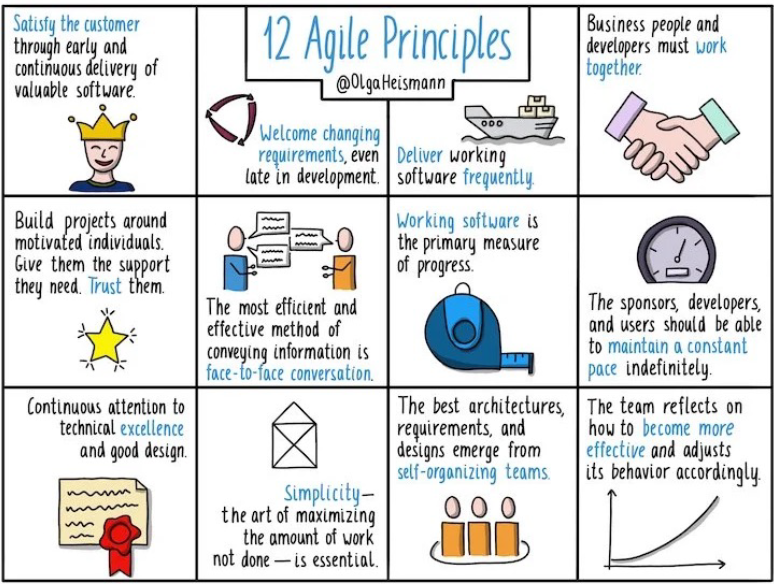
\includegraphics[scale=0.5]{20}
\end{center}

Ver analogia nos slides 6 a 15.

\pagebreak

\subsection{Técnicas de Desenvolvimento Agile}

As fases especificação, design, implementação e avaliação são intercaladas:
\begin{itemize}
  \item O sistema é desenvolvido  como uma série de versões, envolvendo
  \textbf{stakeholders} na especificaçãon e avaliação;
  \item Entregas de novas versões frequente para avaliação;
\end{itemize}

Vasto suporte de ferramentas (ex: ferramentas de testes automáticos) usado
para suportar o desenvolvimento.

\vspace{2mm}

Miníma documentação, uma vez que o foco é o código.

\begin{center}
  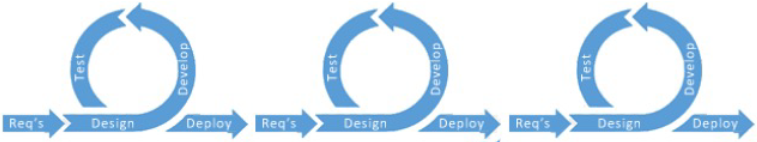
\includegraphics[scale=0.5]{21}
\end{center}

\subsubsection{Extreme Programming (XP)}

Extreme Programming (XP) é a abordagem mais utilizada para desenvolvimento
ágil de software. \textbf{Leva uma abordagem "extrema" para o desenvolvimento iterativo}:
\begin{itemize}
  \item Novas versões podem ser contruidas varias vezes por dia;
  \item Os incrementos são entregues aos clientes \uline{a cada 2 semanas};
  \item Todos os testes devem correr para cada build e cada buid apenas é aceite
  se todos os testes correrem com sucesso;
\end{itemize}

\vspace{2mm}

Utiliza uma abordagem orientada a objetos como o paradigma de desenvolvimento
preferido. Abrange um conjunto de regras e práticas que
ocorrem no contexto de quatro atividades fundamentais (framework activities):
\textbf{planning, design, coding, testing}.

\subsubsection{Release Cycle XP}

\begin{center}
  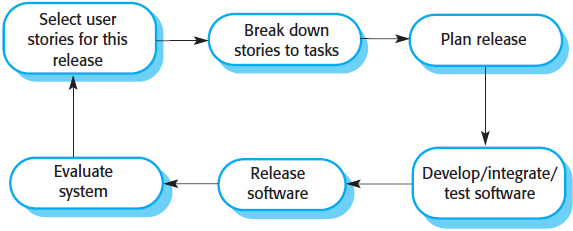
\includegraphics[scale=0.55]{22}
\end{center}

\pagebreak

\subsubsection{Práticas XP}

\begin{center}
  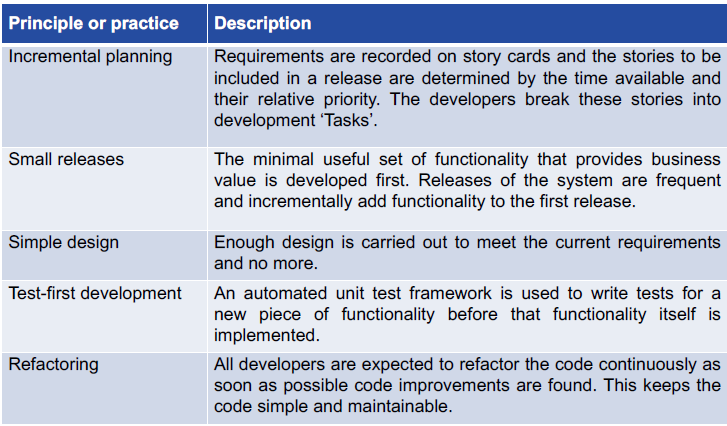
\includegraphics[scale=0.45]{23}
  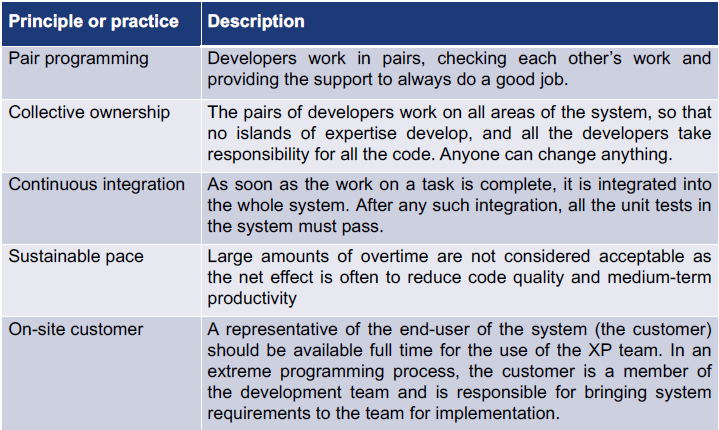
\includegraphics[scale=0.45]{24}
\end{center}

\subsubsection{Práticas influentes de XP}

Extreme Programming tem um foco técnico e não é fácil de integrar
com prática de gestão na maior parte das organizações.
Consequentemente, enquanto desenvolvimento Agile utiliza práticas
de XP, o método referido não é muito utilizado.

\vspace{2mm}

Práticas Chave:
\begin{itemize}
  \item User stories para especificação;
  \item Refatoração;
  \item Desenvolvimento Test-First;
  \item Programação em pares (pair programming);
\end{itemize}

\subsubsection{User Stories para Requisitos}

Em XP, o cliente ou user são parte da equipa XP e são
\textbf{responsáveis por tomar decisões sobre requisitos}.

\vspace{2mm}

Requisitos do user são expressos como \textbf{user stories} ou
\textbf{scenarios}. Estes são escritos em cartões e a equipa
de desenvolvimento divide-os em \textbf{tarefas de implementação}.
Estas tarefas são a base das estimativas de custo e de schedule.

\vspace{2mm}

O cliente escolhe as \textbf{stories para inclusão} na próxima release
baseado em prioridade e estimativa de schedule.

\vspace{2mm}

Exemplo slide 24 e 25.

\pagebreak

\subsubsection{Templates de User Stories}

\begin{center}
  As a \textbf{(user)}, I \textbf{(want to)}, \textbf{(so that)}.
\end{center}

\begin{itemize}
  \item \textbf{User:} Refere o user final do software;
  \item \textbf{Want to:} Refere à intenção do user, e não
  à feature que este utiliza. Temos de especificar aquilo que
  o user quer alcançar com a tarefa, sem mencionar a UI da aplicação;

  \item \textbf{So that:} Descreve a "bigger picture". Qual é o objetivo
  do user? O que é que ele quer alcançar com esta feature?
\end{itemize}


\begin{flushleft}
  \textbf{Exemplo:} As a \uline{manager}, I want to be able to
  \uline{understand my colleagues progress} so that I can
  \uline{report our success and failures}.
\end{flushleft}

\subsubsection{Organização de User Stories}

\begin{itemize}
  \item \textbf{Role-Goal-Benefit:} Força o cliente a realmente pensar
  quem é que vai beneficiar de uma feature, o que é que eles querem
  alcançar e porque é que eles querem alcançar isso;

  \item \textbf{Limites/Needs:} Subconjunto de situações que são de interesse para esta feature;
  \item \textbf{Definição de Done:} Como validar uma feature e saber que esta está concluida?
  \item \textbf{Tarefas de Engenharia:} Como esta feature interaje com outras features
  dentro do sistema ou outros subsistemas;
  \item \textbf{Estimativa de esforço:} Fornece uma medida concreta sobre o valor de uma feature;
\end{itemize}

\subsubsection{Refatoração}

Conhecimento convencional em engenharia de software é \textbf{design for change}.
Compensa gastar tempo e esforçarmo-nos a anticipar mudanças, uma vez que,
reduz o cussto mais à frente no ciclo de vida.

\vspace{2mm}

No entanto, XP mantém que este principio não compensa, uma vez que,
mudanças não podem ser previstas. Em vez disso, propõe
\textbf{melhorias contantes do código} (refactoring) para tornar
mudanças mais fáceis quando têm de ser implementadas.

\vspace{2mm}

Equipas de programação procuram por possíveis \textbf{melhorias de software}
e fazem-nas mesmo que não sejam necessárias naquele momento.
Isto melhora a \textbf{compreensão do software} e desta maneira reduz
a necessidade de documentação.

\vspace{2mm}

Mudanças são \textbf{fáceis de fazer} uma vez que o código é
\textbf{bem estruturado} e \textbf{claro}. No entanto, algumas mudanças
requerem \uline{architecture refactoring}, o que é muito mais caro.

\subsubsection*{Exemplo}

\begin{itemize}
  \item \textbf{Re-organização} de uma classe hierárquica para remover duplicação de código;
  \item \textbf{Renomear} atributos e métodos de modo a serem mais faceis de entender;
  \item \textbf{Trocar inline code} com chamadas de métodos que estão incluidas em bibliotecas;
\end{itemize}

\pagebreak

\subsubsection{Desenvolvimento Test-First}

Testar é uma parte central em XP. O \textbf{desenvolvimento test-first}:
\begin{itemize}
  \item Teste incremental é desenvolvido a partir de cenários;
  \item Envolvimento de users no desenvolvimento de testes e validação;
  \item Correr todos os testes de componente de cada vez que uma nova versão
  é built.
\end{itemize}

\begin{center}
  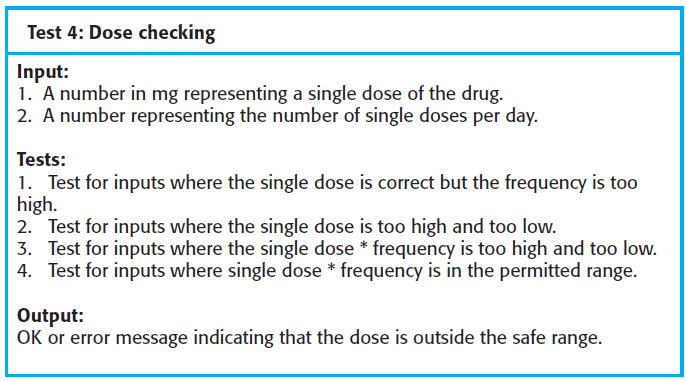
\includegraphics[scale=0.5]{25}
\end{center}

\subsubsection{Automação de Testes}

Testes são escritos como \textbf{componentes executáveis} antes da
tarefa ser implementada. Estes devem:
\begin{itemize}
  \item Ser autonomos (stand-alone);
  \item Simular a submissão de input para ser testado;
  \item Verificar que o resultado é o esperado;
\end{itemize}

Uma \textbf{automated test framework} (ex: Junit) torna mais fácil
de escrever e executar testes.

\vspace{2mm}

Uma vez que os testes são automáticos, existe um conjunto de testes
que podem ser rapidamente e facilmente executados. Quando uma nova
funcionalidade é adicionada ao sistema, todos os testes podem ser executados
e identificar problemas no novo código imediatamente.

\subsubsection{Problemas com o desenvolvimento Test-First}

\begin{itemize}
  \item Os programadores preferem programar em vez de escrever testes,
  pelo que, por vezes estes fazem \textbf{short cuts ao escrever testes}.
  Como pro exemplo, testes incompletos que não testam todas as possibilidades.

  \item Alguns testes são \textbf{muito difíceis de escrever incrementalmente}.
  Como testes para uma UI complexa, é difícil escrever testes com display logic.

  \item É dificil de julgar a \textbf{cobertura} de um conjunto de testes.
  Podemos ter muitos testes de sistema e não cobrir tudo.
\end{itemize}

\pagebreak

\subsubsection{Programação em Pares (Pair Programming)}

Um parte programadores a trabalharem juntos para desenvolver código.
Os programadores sentam se juntos num mesmo computador para desenvolver
software. Serve como uma forma de \textbf{revisão de código informal}
uma vez que cada linha de código é olhada por mais do que uma pessoa.

\vspace{2mm}

Isto ajuda a desenvolver \uline{common ownership} do código e
\uline{compreensão coletiva} pela equipa.
Reduz o risco quando um programador deixa a equipa.

\vspace{2mm}

Em pair programming, os pares são criados dinamicamente
para que todos os membros da equipa trabalhem uns com os outros durante
o processo de desenvolvimento. Encoraja a refatorização, uma vez que,
toda a equipa pode benificiar com a melhoria do código do sistema.

\vspace{2mm}

Pair programming não é necessariamente ineficiente. Estudos mostram
que um par ao trabalhar junto é mais eficiente do que dois programadores
a trabalhar separadamente.

\subsection{Gestão de Projeto Agile}

A principar responsabilidade da gestão de projeto de software é
\textbf{gerir o projeto}, para que o software \uline{seja entregue a tempo}
e dentro do \uline{budget} planeada para o projeto.

\vspace{2mm}

A abordagem tradicional para a gestão de projeto é \textbf{plan-driven}.
Define \uline{o que} deve ser entregue, \uline{quando} deve ser entregue e \uline{quem}
vai trabalhar em cada entrega.

\vspace{2mm}

A gestão de projeto Agile requer uma abordagem diferente.
É adaptada de um \textbf{desenvolvimento incremental} e as \textbf{praticas
usadas em métodos agile}.

\subsubsection{Scrum}

É um \textbf{método agile} que foca na gestão incremental do desenvolvimento.

\vspace{2mm}

Existem três fases no Scrum:
\begin{itemize}
  \item A fase inicial é o \textbf{outline planning} onde tem de se estabelecer
  os objetivos gerais para o projeto e fazer o design da arquitetura
  de software.

  \item Isto é seguido por uma serie de \textbf{ciclos sprint}, onde cada
  ciclo desenvolve um incremento do sistema.

  \item A fase de \textbf{encerramento do projeto}, termina o projeto,
  completa a documentação necessária como ajudas nos frames e manual do
  utilizador e acessa aquilo que foi aprendido com o projeto.
\end{itemize}

\begin{center}
  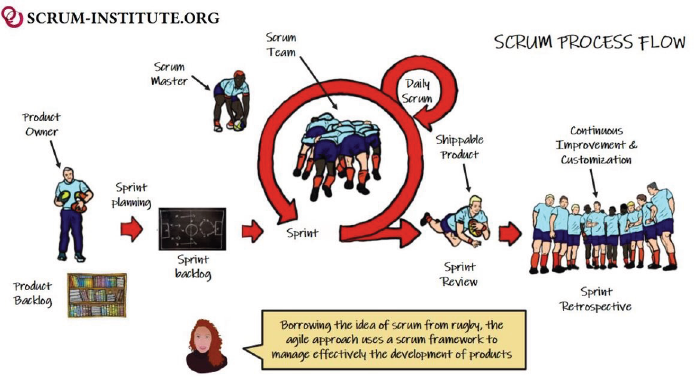
\includegraphics[scale=0.45]{26}
\end{center}

\pagebreak

\subsubsection{Scrum - Terminologia}

\begin{center}
  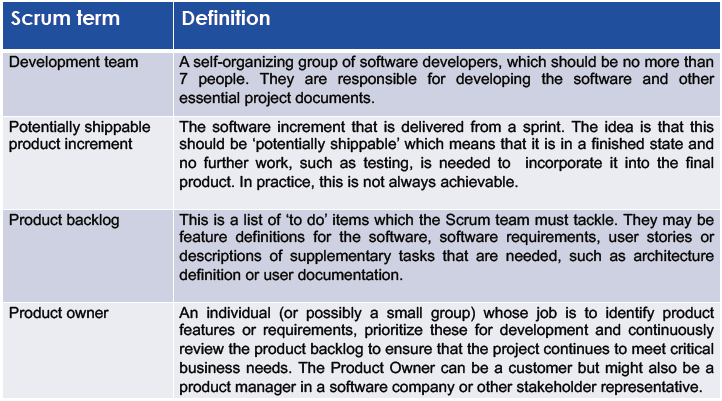
\includegraphics[scale=0.45]{27}
  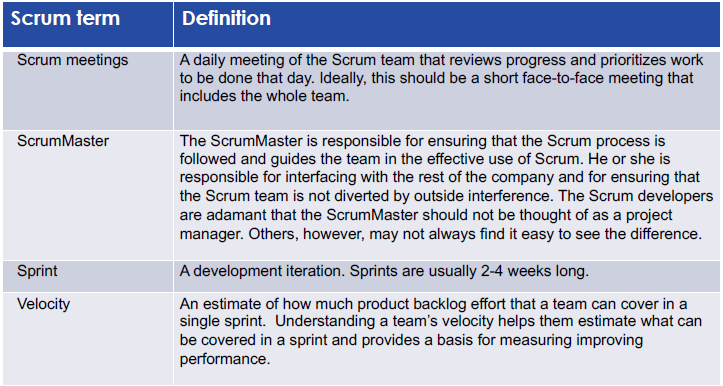
\includegraphics[scale=0.45]{28}
\end{center}

\subsubsection{Scrum sprint cycle}

\begin{center}
  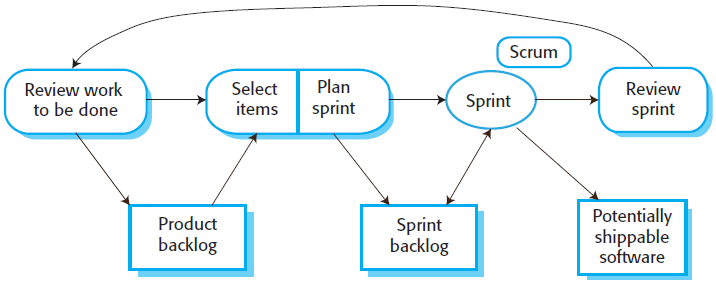
\includegraphics[scale=0.5]{29}
\end{center}

O ponto inicial ara o planeamento é o \textbf{product backlog}.
É uma lista do trabalho a ser feito no projeto.

\vspace{2mm}

A \textbf{fase selecionada} envolve toda a equipa. Quem trabalha com o
cliente para selecionar as features e as funcionalidades do
\textbf{product backlog} que vão ser desenvolvidas durante o sprint.

\vspace{2mm}

Durante a \textbf{fase de desenvolvimento}, a equipa está isolada do
cliente e da organização. Todos os canais de comunicação passam pelo
"\textbf{Scrum master}".

\vspace{2mm}

No \textbf{final do sprint}, o trabalho realizado é revisto e apresentado aos
stakeholders.

\subsubsection{Teamwork in Scrum}

O papel do \textbf{Scrum master} é proteger o a equipa de desenvolvimento
de distrações externas.
\begin{itemize}
  \item Realiza reuniões diárias;
  \item Vai verificando o backlog para ver o trabalho a ser feito;
  \item Toma decisões;
  \item Mede o progresso usando o backlog;
  \item Comunica cocm os clientes e a gestão fora da equipa;
\end{itemize}

A equipa vai a reuniões diárias curtas (\textbf{Scrums})
\begin{itemize}
  \item Membros partilham informação, descrevem o progresso/problemas
  desde a última reunião, e aquilo que estava planeado para o dia;

  \item Isto significa que todos na equipa sabem aquilo que se passa,
  os porblemas que surgiram, podem re-planear num curto tempo o trabalho;
\end{itemize}

\subsubsection{Scrum - Benefícios}

\begin{itemize}
  \item O produto é repartido num conjunto de pedaços \textbf{geriveis}. e \textbf{faceis de compreender}.
  \item \textbf{Requisitos instáveis} não prrendem o progresso;
  \item Toda a equipa tem visibilidade de tudo, consequentemente, a comunicação da equipa melhora;
  \item Os clientes vêm as entregas on-time dos incrementos, ganhando feedback em como o produto funciona;
  \item Confiança entre a equipa e o cliente, todos esperam que o projeto tenha sucesso;
\end{itemize}

\subsubsection{Kanban}

É um sistema ágil que pode ser usado para melhorar qualquer desenvolvimento
de software incluindo Scrum, XP ou Waterfall.

\vspace{2mm}

O nome "Kanban" vem do Japonês e significa "signboard" ou "billboard".
Foi usado pela primeira vez pela Toyota para Just-in-time manufacturing
plants, com o objetivo de limitar o trabalho em progresso (WIP - work in progress).

\subsubsection{Scrum vs Kanban}

Em \textbf{Scrum}, tu escolhes o trabalho que vais fazer durante o
próximo sprint antes deste começar. Depois, damos \uline{lock}
ao sprint, fazemos o trabalho todo, e passado algumas semanas
(duração normal para um sprint), a queue fica vazia.

\begin{center}
  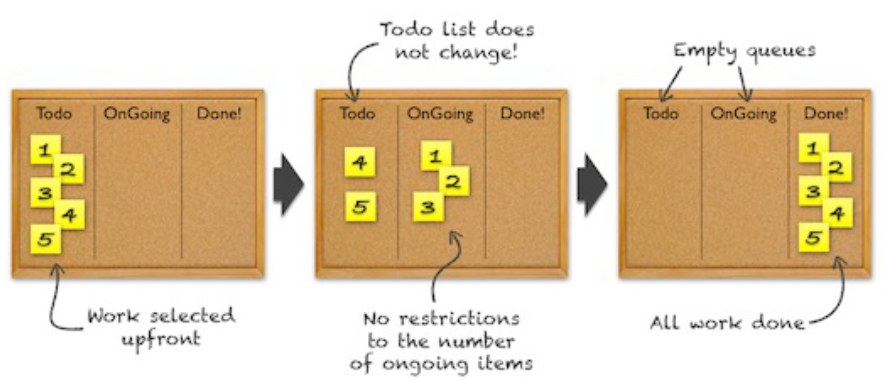
\includegraphics[scale=0.48]{30}
\end{center}

Em \textbf{Kanban}, tudo o que é limitado é o tamanho das queues,
chamado de \textbf{work in progress (WIP) limits}. Podemos alterar
os items na queue a qualquer momento, não existindo
um "fim de sprint". O trabalho continua a fluir.  

\begin{center}
  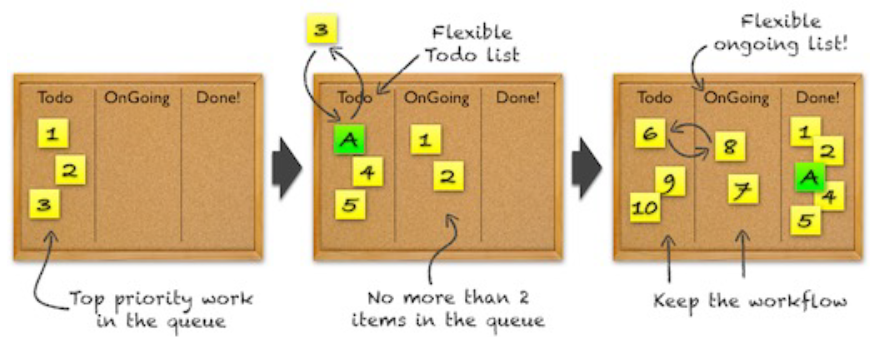
\includegraphics[scale=0.48]{31}
\end{center}


\pagebreak

\begin{center}
  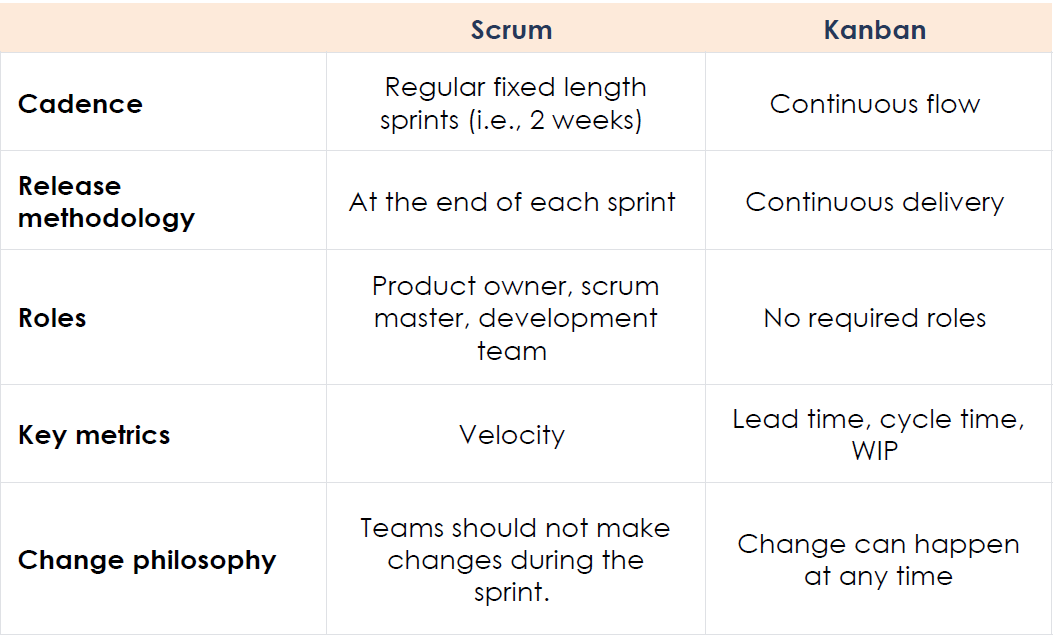
\includegraphics[scale=0.4]{32}
\end{center}

\subsection{Scaling Agile Methods}

Métodos Agile provaram ser muito eficazes para projetos
pequenos/médios, que podem ser desenvolvidos por uma equipa
pequena co-localizada.
Escalar métodos Agile involve mudar estes para poderem ser
utilizados em projetos cada vez maiores, onde existem múltiplas
equipas de desenvolvimento, podendo trabalhar até mesmo em diferentes
locais.

\vspace{2mm}

Quando escalamos métodos Agile, é importante manter fundamentos
Agile: Planeamento flexivel, releases de sistema frequentes,
integração contínua, desenvolvimento test-driven e boa comunicação
entre a equipa.

\subsubsection{Problemas de Sistema}

\begin{itemize}
  \item Quão grande é o sistema a ser desenvolvido? Métodos Agile
  \uline{são mais eficientes em equipas pequenas e co-localizadas}, em que
  ocorre uma comunicação informal.

  \item Que tipo de sistema está a ser desenvolvido? Sistemas que necessitem
  de \textbf{muita análise antes da implementação} precisam de um
  design (mais) detalhado.

  \item Qual é o tempo de vida esperado do sistema?
  \textbf{Sistemas de longa duração necessitam de documentação} para comunicar
  as intenções do sistema com os developers da equipa de suporte.

  \item O sistema está sujeito a regulamentos externos?
  Se o sistema é regulado, muito provavelmente, é necessário
  \textbf{produzir documentação detalhada} como parte do caso de segurança do
  sistema.
\end{itemize}

\subsubsection{Desenvolvimento de Sistemas Grandes}

Sistemas grandes são normalmente coleções de sistemas de comunicação separados,
onde \textbf{equipas separadas} desenvolvem cada sistema. Frequentemente,
estas equipas trabalham em locais diferentes, por vezes até em zonas com diferentes fusos horários.

\vspace{2mm}

Sistemas grandes são "\textbf{brownfield systems}" isto é,
incluem e interagem com vários sistemas existentes.
Muitos dos requisitos do sistema estão relacionados com a interação, logo
não se rendem muito à flexibilidade e desenvolvimento incremental.

\pagebreak

Sistemas grandes e os seus processos de desenvolvimento são
muitas vezes restritos por \textbf{regras e regulamentos externos},
limitando a forma como podem ser desenvolvidos.

\vspace{2mm}

Sistemas grandes tem uma \textbf{aquisição longa} e
um tempo de desenvolvimento longo também. É dificil de manter equipas
coerentes que sabem sobre o sistema durante esse periodo, uma vez que,
eventualmente, os membros vão para outros projetos ou trabalhos.

\vspace{2mm}

Sistemas grandes normalmente tem um conjunto diverso de
\textbf{stakeholders}. É praticamente impossível involver todos estes
stakeholders no processo desenvolvido.

\subsubsection{Agile: Scaling up em sistemas grandes}

\begin{itemize}
  \item Uma \uline{abordagem completamente incrementeal aos requisitos de engenharia} é \textbf{impossível};
  \item \textbf{Não pode existir} um único \uline{product owner};
  \item \textbf{Não é possível} \uline{focar apenas no código};
  \item \uline{Mecanismos de comunicação cross-team} têm de ser \textbf{designed} e \textbf{utilizados};
  \item \uline{Integração continua} é praticamente \textbf{impossível}, no entanto, é essencial
  manter builds frequentes do sistema e regular releases do sistems;
\end{itemize}

\subsubsection{Multi-team Scrum}

\begin{itemize}
  \item \textbf{Role replication}: Cada equipa tem um Product Owner para o
  seu trabalho e Scrum Master.

  \item \textbf{Product architects}: Cada equipa escolhe um arquiteto
  do produto que colaboram para desenhar e evoluir toda a arquitetura
  do sistema.

  \item \textbf{Release alignment}: As datas de releases de produtos
  de cada equipa são alinhadas de modo a demonstrar que um sistema
  completo está produzido.

  \item \textbf{Scrum of scrums}: Existe um Scrum of scrums diário, onde
  os representantes de cada equipa se encontram para discutir o progresso
  e o plano de trabalho a ser concluído.
\end{itemize}

\pagebreak

\section{DevOps}

\subsection{Metodologia Agile}

\begin{itemize}
  \item Cada projeto é dividido em várias iterações;
  \item Todas as iterações devem ter a mesma duração (2-8 semanas);
  \item No final de cada iteração, um produto funcional deve ser entregue;
\end{itemize}

\begin{center}
  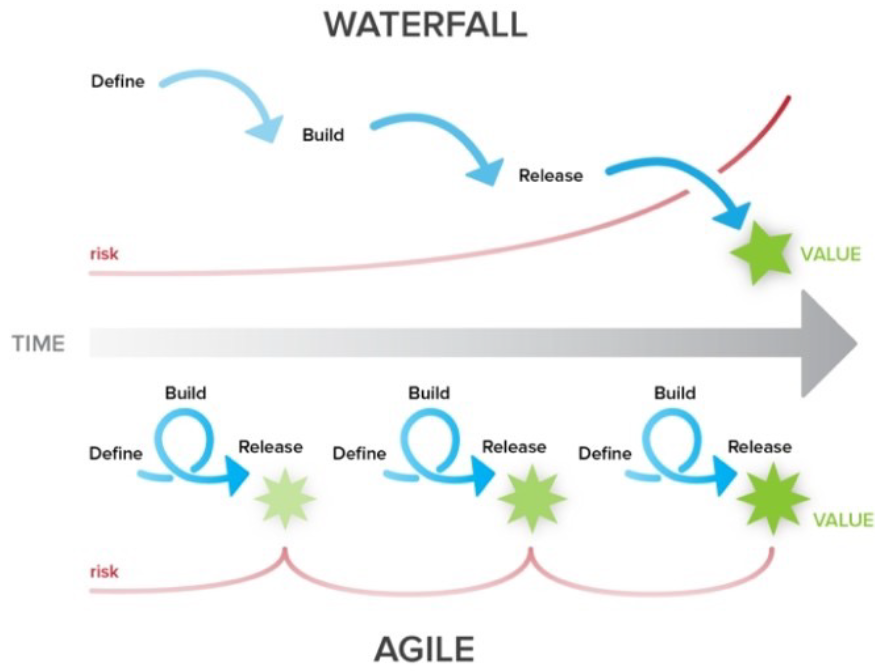
\includegraphics[scale=0.45]{33}
\end{center}

\subsection{Quais são as limitações de Agile?}

Enquanto que a parte de Desenvolvimento é continua,
a parte de Operações não é.

\begin{center}
  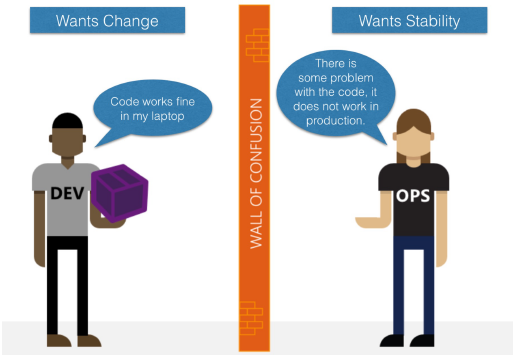
\includegraphics[scale=0.6]{34}
\end{center}


\subsection{Dev vs Ops}

A equipa de \textbf{desenvolvimento} começa a trabalhar no projeto,
"atirando" uma realease de software "por cima da parede" para as
Operações.

\vspace{1mm}

As \textbf{Operações} pegam nos artefactos da release e começam
a preparar o seu desenvolvimento. Estes também  editam os ficheiros
de configuração para refletir o ambiente de produção
(que é \textbf{bastante diferente dos ambientes de Desenvolvimento}).

\pagebreak

Em caso de falha\dots
\begin{itemize}
  \item Os Developers são chamados para resolver o problema;
  \item \textbf{Operações} afirma que \uline{O Desenvolvimento
  deu código defeituoso};
  \item \textbf{Desenvolvimento} responde apontando o facto de que
  \uline{funcionava perfeitamente nos seus ambientes}
  (logo o problema é das Operações, que fizeram algo de errado).
  \item Os Developers estão a ter dificuldades em sequer perceber o problema.
  Devido à configuração, localização dos ficheiros, ao procedimento utilizado
  para chegar a esse estado é diferente do esperado.
\end{itemize}

\begin{center}
  \textbf{Qual é a Solução?}
\end{center}

\subsection{DevOps}

DevOps é sobre a remoção das barreiras entre duas equipas
tradicionalmente isoladas: \textbf{Desenvolvimento} e \textbf{Operações}.

\vspace{2mm}

Em algumas organizações, pode nem haver uma equipa separada,
\textbf{os engenheiros fazem ambos}.

\vspace{2mm}

As \textbf{duas equipas trabalham juntas} de modo a otimizar
tanto a produtividade dos desenvolvedores e a fiabilidade
das operações.
Estas \textbf{comunicam frequentemente} aumentando a eficiência
e a qualidade dos serviços que fornecem aos clientes.

Têm um \textbf{ownership completo para os seus serviços}, pensando
nas necessidades dos clientes finais e como podem contribuir para
resolver essas necessidades.

\vspace{2mm}

As equipas vêm o ciclo completo de desenvolvimento e infrastruturas
como parte das suas responsabilidades.

\begin{center}
  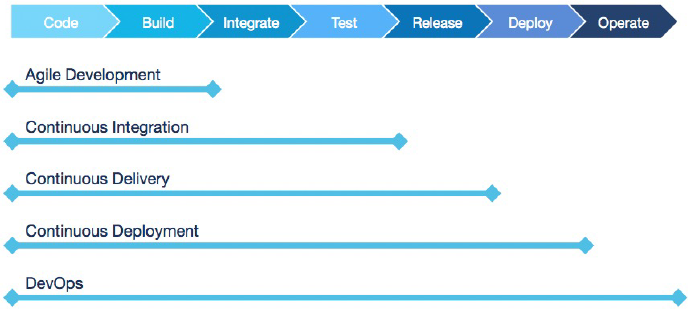
\includegraphics[scale=0.6]{35}
\end{center}

\pagebreak

\begin{itemize}
  \item \textbf{Desenvolvimento} Agile. Gestão do código fonte
  (Plan, Code, Build). Manutenção de diferentes versões do código;
  \item \textbf{Integração} Contínua (Integrate, Test).
  Compilar, revisão de código, testes unitários, testes de integração;
  \item \textbf{Entrega} Contínua (Release). Deploy da aplicação (build), realizando
  testes de aceitação nos users;
  \item \textbf{Desenvolvimento} Contínuo (Deploy, Operate). Deploy na
  aplicação testada/aceite;
  \item \textbf{Monitorização} Contínua;
\end{itemize}

\subsubsection{DevOps - Ciclo de Vida}

\begin{center}
  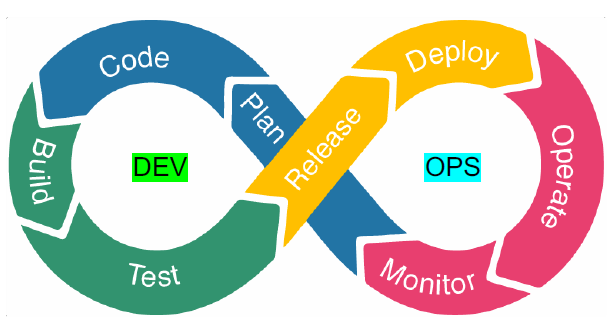
\includegraphics[scale=0.55]{36}
\end{center}

\subsubsection{DevOps - Como implementar?}

\begin{center}
  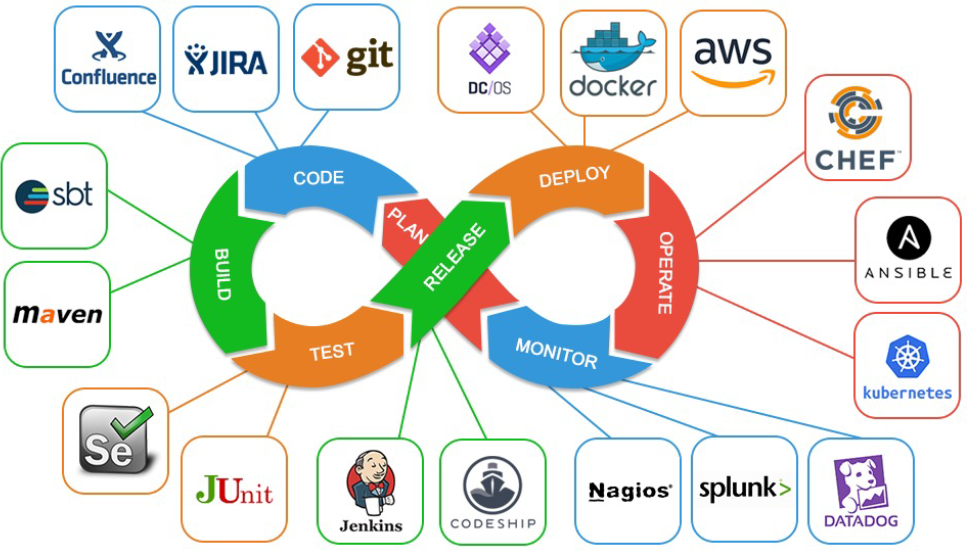
\includegraphics[scale=0.55]{37}
\end{center}

\pagebreak

\subsection{Um asset chave: Infrastrutura como Código (IaC)}

\textbf{a.k.a. Programmable Infrastructure} ou \textbf{software-defined
infrastructure}
\begin{itemize}
  \item A infrastrutura é decrita por código e pode ser trackeada,
  validada, e reconfigurada de forma automática;
  \item Engenheiros DevOps podem interagir com a infraestrutura utilizando
  ferramentas code-based e \textbf{tratando a infrastrutura de uma
  forma semelhante a como tratam o código da aplicação};
\end{itemize}

\vspace{2mm}

Gestão de configuração
\begin{itemize}
  \item Developers e administradores de sistemas usam código para
  \uline{automar sistemas operativos} e \uline{configurar hosts},
  \uline{tarefas operacionais}, e mais;
  \item A utilização de código faz com que as mudanças na configuração
  sejam \uline{repetíveis} e \uline{padronizadas};
\end{itemize}

\subsection{Integração Contínua (CI)}

\subsubsection{Ideia base de CI}

A continua integração é um processo onde o código é
verificado para um repositório frequentemente.

\begin{center}
  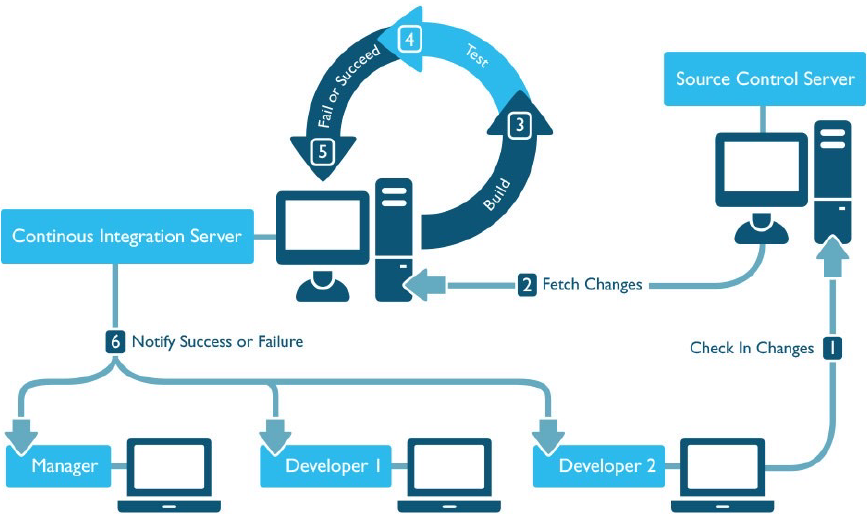
\includegraphics[scale=0.55]{38}
\end{center}

\pagebreak

\subsubsection{Poruque é que CI é crucial para DevOps?}

\begin{flushleft}
  \textbf{Erros são encontrados mais cedo:}
  \begin{itemize}
    \item Se existe um erro na cópia local ou no código,
    uma falha na build vai ocorrer no "estado apropriado";
    \item Força o desenvolvedor a corrigir o bug antes de
    proceder. Equipas QA (Quality Assurance) vão também beneficiar
    disto, uma vez que estas vão trabalhar mais frequentemente em builds estáveis;
  \end{itemize}

  \textbf{Definir o estágio para CI/CD:}
  \begin{itemize}
    \item CI reduz interveenção manual, uma vez que a build,
    sanidade e outros testes são supostamente executados automaticamente;
    \item Isto permite uma entrega continua de sucesso
  \end{itemize}

  \textbf{Confidencialidade do Projeto}
\end{flushleft}

\subsubsection{Getting Started with CI}

\begin{itemize}
  \item \textbf{Build Script} (ex: Maven, Gradle, Ant, Make, \dots),
  é um script, ou um conjunto de scripts, usados para compilar, testar,
  inspecionar e dar deploy a um software;

  \item \textbf{Version Control System} (ex: Git, GitHub, GitLab, \dots),
  permite guardar todas as mudanças feitas a um ficheiro ou conjunto
  de ficheiros ao longo do tempo, de modo a que seja possível
  aceder a versões específicas mais tarde;

  \item \textbf{CI Server} (ex: Jenkins, Travis CI, Hudson, \dots),
  é um servidor que corre uma build de integração quando uma mudança
  é commited num repositório de controlo de versões. Apesar de ser recomendado
  correr uma build a cada mudança, buikds podem ser agendadas
  (ex: nightly builds);

  \item \textbf{Automation testing framework} (ex: Selenium, Appium,
  TestComplete, \dots);
\end{itemize}

\subsubsection{Build Script com Maven}

\vspace{2mm}

\begin{center}
  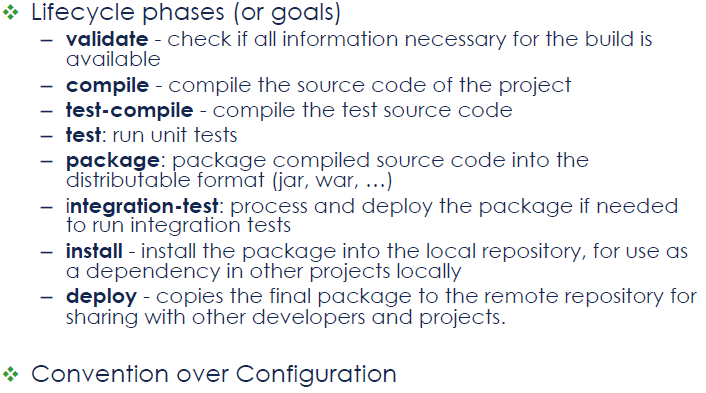
\includegraphics[scale=0.55]{39}
\end{center}

\pagebreak

\subsubsection{CI Server com Jenkins}

O \textbf{código é built} e testado quando um desenvolvedor
faz um commit. Se o build for bem sucedida,
\textbf{Jenkins faz deploy} da fonte para um servidor de testes
e notifica a equipa de deployment.
Se a build falhar, então o Jenkins vai notificar os erros
à equipa de desenvolvimento.

\begin{center}
  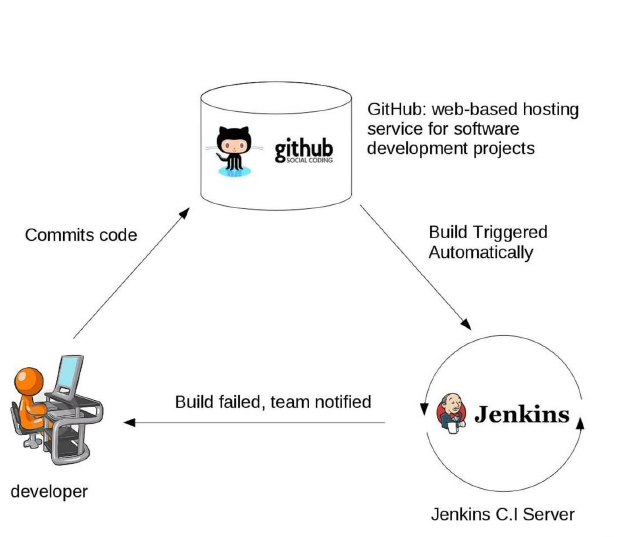
\includegraphics[scale=0.55]{40}
\end{center}

\subsubsection{CI - Best Practices}

\begin{flushleft}
  \textbf{Versioning}
  \begin{itemize}
    \item Repositório partilhado para manter o código. Todos os
    ficheiros donte são commited para o repositório;
    \item Merge diário. As mudanças são commited para a mainline, diariamente;
    \item Short-lived branches. É assim que devem ser, idealmente menos de uns dias
    e nunca mais do que uma iteração;
  \end{itemize}

  \textbf{Build Configuration}
  \begin{itemize}
    \item Build independente. Escrever build scripts desacopolados de IDEs. Estes são executados pelo
    sistema CI para que o software possa ser built a cada mudança;
    \item Build em cada mudança. Building e testar software a cada mudança commited;
    \item Limite de build. Falhar uma build quando uma regra do projeto é violada (ex: testes lentos);
  \end{itemize}

  \pagebreak

  \textbf{Team Policy}
  \begin{itemize}
    \item Stop the line (build quebrada). Corrigir erros de entrega de software mal estes aconteçam;
    \item Fazer commits regularmente. Cada membro da equipa deve verificar o "trunk", pelo menos uma vez por dia;
    \item Feedback continuo. Enviar feedback automaticamente do sistema CI
    para os membros da Cross-functional team;
    \item Falhas rápidas. Falhar a build o mais rápido possível;
    \item Builds rápidas. Uma build fornece feedback em problemas
    comuns o mais rápido possível (normalmente menos de 10 minutos);
  \end{itemize}
\end{flushleft}

\subsection{Entrega Contínua (CD)}

A Engenharia de Software é baseada em \textbf{CI}. CI
foca nas equipas de desenvolvimento, em que o output é o
input do porcesso de testes manuais e o resto do processo
de realease.

Muito tempo pode ser "perdido" desta forma através de testes
e operações (ex: testers esperam por "boas" builds de software
equipas de operações esperam por documentação e fixes).

\vspace{2mm}

\textbf{CD} previne isto, as relações entre stakeholders
involvidos na entrega é mais proxima e colaborativa (cultura DevOps).

Automação extensiva a todas as partes do processo de entrega,
CD pipeline.

\subsubsection{CD Pipeline}

\begin{center}
  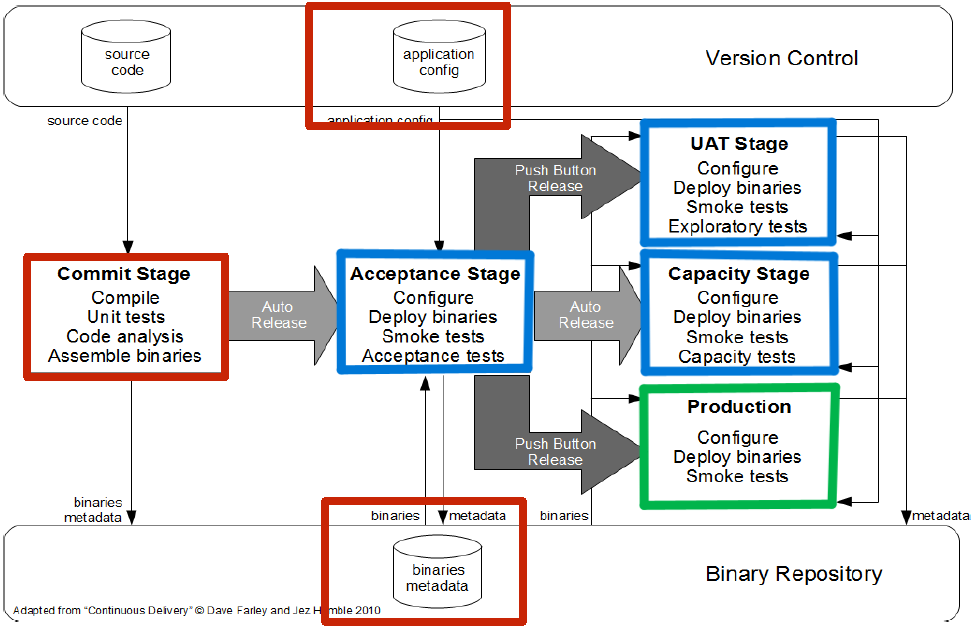
\includegraphics[scale=0.55]{41}
\end{center}

\begin{center}
  \textbf{Vermelhos}: Fase de CI;
  \textbf{Azuis}: Fase pós CI;
  \textbf{Verdes}: Fase de CD;
\end{center}

\pagebreak

\subsubsection*{Fase pós CI}

Consiste de múltiplos ambientes/estágios com o objetivo de testar.
Inclui testes \textbf{manuais e automaticos}.

Alguns estágios podem ser executados em paralelo (ex: user
acceptance testing (UAT) e performance testing em sistemas de backend).

Estágios podem ser automaticamente executados quando o anterior
termina ou é manualmente aprovado (ex: clicar um botão).

\subsubsection*{Fase de CD}

Novas versões estão disponíveis para os clientes.
Existem várias estratégias e práticas para fazer isto:
\begin{itemize}
  \item eat your own dog food;
  \item canary releases;
  \item dark launches;
  \item gradual rollouts;
  \item A/B testing;
  \item blue/green deployments;
\end{itemize}

\subsubsection{Eat your own dog food}

\begin{flushleft}
  \textbf{Ideia:} Os empregados utilizam a versão mais recente internamente.
  Se tudo estiver como esperado, então a versão é lançada para os clientes.

  \vspace{2mm}

  "A companhia usa o seu próprio produto para testar e promover o produto".
\end{flushleft}

\subsubsection{Canary Releases}

\begin{flushleft}
  \textbf{Ideia:} Lançar uma nova versão para um subconjunto de utilizadores
  primeiro, enquando o resto interage com a versão antiga estável.
  Em cado de problemas com esta nova versão, \uline{apenas um pequeno
  número de utilizadores é afetado}, logo o impacto do problema é reduzido. 

  \vspace{2mm}

  Canário é comparado à versão existente em termos do
  conjunto dos critérios como estabilidade, performance, ou correção.
  Os utilizadores são escolhidos com base na sua localização,
  role (ex: admin, early, stable, \dots) e de forma aleatória
  (ex: 1\% dos utilizadores).
\end{flushleft}

\subsubsection{Dark Launches}

\begin{flushleft}
  \textbf{Ideia:} Mitigar problemas de performance e de reliability
  de novas funcionalidades ao enfrentar carga semelhante à de produção,
  através de um lançamento em produção, \uline{sem ser visivel para os utilizadores}.

  \vspace{2mm}

  Dark launches são normalmente released para um \uline{grupo de
  utilizadores que não sabem que estão a ser testados}. A nova funcionalidade
  não lhes é indicada de qualquer maneira.

  Dev teams podem identificar e corrigir os erros restantes.
  Preocupações de escalabilidade antes de habilitar a funcionalidade para os utilizadores.
\end{flushleft}

\pagebreak

\subsubsection{Gradual Rollouts}

\begin{flushleft}
  \textbf{Ideia:} \uline{Aumentar o número de users escolhidos}
  para a nova versão de uma forma gradual, até substituir completamente
  a versão antiga.

  Mostra se a nova versão pode lidar com
  aumentando a carga e se escala corretamente.

  \vspace{2mm}

  Muitas das vezes é combinada com \textbf{canary releases} e
  \textbf{dark launches}.
\end{flushleft}

\begin{center}
  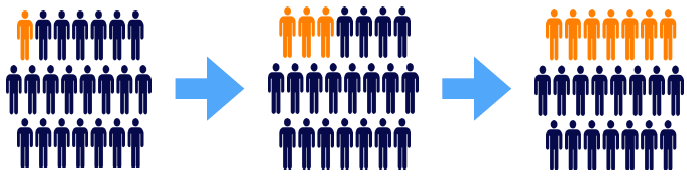
\includegraphics[scale=0.4]{42}
\end{center}

\subsubsection{A/B Testing}

\begin{flushleft}
  \textbf{Ideia:} Comparar \uline{duas versões de software}
  uma à outra, normalmente apenas diferencia num aspeto
  testado, para determinar o efeito de uma dada mudança
  \begin{itemize}
    \item forma estatistica de testar hipoteses, pelo que
    requerem amostras grandes o suficiente para ter "poder estatistico";
    \item maioritariamente usado no UI para testar varios layouts ou
    designs;
  \end{itemize}
\end{flushleft}

\begin{center}
  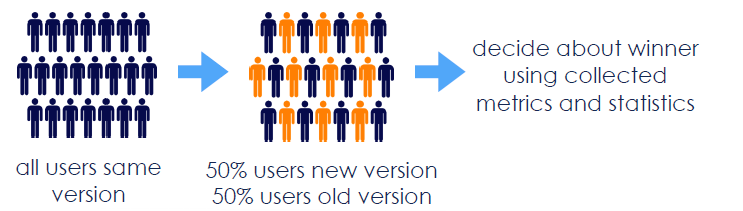
\includegraphics[scale=0.45]{43}
\end{center}

\subsubsection{Blue/Green Deployments}

\begin{flushleft}
  \textbf{Ideia:} ter dois ambientes de produção idênticos,
  um hospedando a versão atual do software (green), versão estável,
  a outra (blue) representa a nova versão.

  \begin{itemize}
    \item \uline{Release:} simplesmente mudar o roiter para que todo o tráfego
    seja direcionado para o ambiente blue (ou green) e utilizar o
    ambiente green (ou blue) para testar a nova versão;
    \item \uline{Vantagens:} em caso de problemas depois da release,
    um rápido rollback (switch) para a versão anterior é possível;
    \item \uline{Obstaculo:} As bases de dados fazem parte de ambos
    os ambientes, pelo que um switch requer uma migração de dados
    / sincronização da base de dados;
  \end{itemize}
\end{flushleft}

\begin{center}
  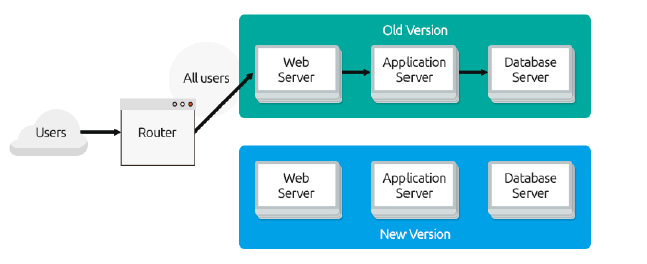
\includegraphics[scale=0.5]{44}
\end{center}

\pagebreak

\subsection{Beneficios de DevOps}

\begin{flushleft}
  \textbf{Velocidade}
  \begin{itemize}
    \item \textbf{Mover a elevada velocidade} de forma a inovar mais rápido
    para os clientes, adaptar as mudanças nos mercados de forma melhor, e
    crescer mais eficientemente em obter resultados de negócio;
    \item Por exemplo, CD deixam as equipas ter ownership
    dos serviços e depois dar release a updates para ser mais rápido;
  \end{itemize}

  \textbf{Fiabilidade}
  \begin{itemize}
    \item Garante a \textbf{qualidade dos updates da aplicação}
    e as mudanças de infrastrutura para poder entregar fiavelmente
    a um ritmo mais rápido, enquanto se mantém uma experiência
    positiva para o cliente;
    \item Usar práticas como \uline{CI e CD para testar cada alteração
    é funcional e seguro};
  \end{itemize}

  \textbf{Escala}
  \begin{itemize}
    \item Automação e consistência \textbf{ajudam a gerir sistemas complexos
    ou com mudanças frequentes} eficientemente e com risco reduzido;
    \item Por exemplo, \uline{infrastruturas como código} ajuda a gerir
    o desenvolvimento, testar, e ambientes de produção de forma
    repetivel e mais eficiente;
  \end{itemize}

  \textbf{Melhora a colaboração}
  \begin{itemize}
    \item \textbf{As equipas de Dev e Ops} colaboram,
    partilham muitos responsabilidades e combinam os seus workflows;
    \item Isto reduz ineficiências e salva tempo, escrevendo código,
    e a reduz a passagem de informação entre equipas;
  \end{itemize}

  \textbf{Segurança}
  \item Mover rapidamente enquando mantém o controlo e preserva a conformidade;
  \item Um pode adotar o modelo DevOps sem sacrificar a segurança através de
  \textbf{politicas automaticas de compliance}, controlos fine-grained e
  configuração de técnicas de gestão;
  \item Por exemplo, usar infrastruturas como código (e politica como
  código), podemos definir e depois rastrear a conformidade em escala;
\end{flushleft}

\pagebreak

\subsection{DevOps - CALMS}

DevOps não é puramente técnico, também inclui aspetos sumarizados
pelo acrónimo \textbf{CALMS}:

\begin{center}
  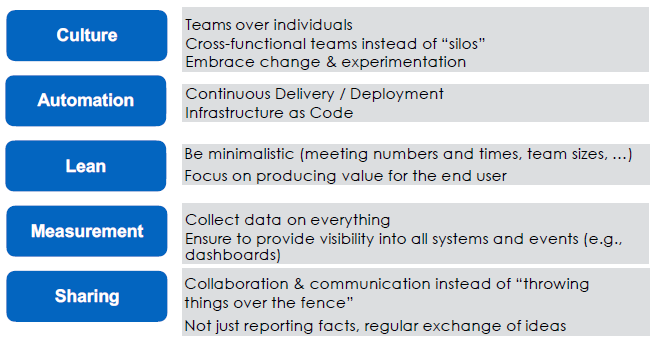
\includegraphics[scale=0.6]{45}
\end{center}

\section{Clean Project}

\subsection{Engenharia de Software - Rever}

\begin{enumerate}
  \item Processo de desenvolvimento de software
  \begin{itemize}
    \item Modelo sequencial (waterfall)
    \item Modelo incremental
    \item Modelo evolutivo/iterativo
  \end{itemize}

  \item Metodologias de desenvolvimento Agile
  \begin{itemize}
    \item Princípios Agile e gestão de projeto
  \end{itemize}

  \item DevOps, benefícios técnicos
  \begin{itemize}
    \item Entrega de software contínua
    \item Entregas de features mais rápidas (time to market)
  \end{itemize}
\end{enumerate}

\subsection{Papéis}

\begin{center}
  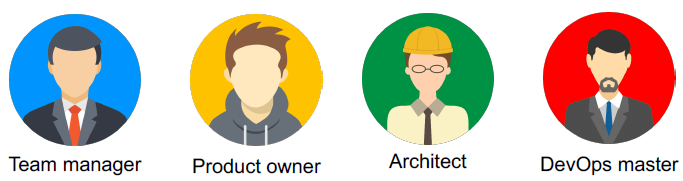
\includegraphics[scale=0.6]{46}
\end{center}

\pagebreak

\subsubsection{Team Manager}

\begin{itemize}
  \item Modera as discussões (reuniões) da equipa. Promove a colaboração
  dentro da equipa e toma iniciativa para resolver problemas;
  \item Gere e atribui as tarefas;
  \item Pode ser visto como um Scrum Master;
  \item \textbf{Responsável por entregar os outcomes do projeto a tempo};
\end{itemize}

\subsubsection{Product Owner}

\begin{itemize}
  \item Representa os interesses dos stakeholders;
  \item Sabe aquilo que a aplicação deve fazer (features, requisitos, user stories);
  \item Responsável por aceitar os incrementos da solução. Deve rever novas releases;
\end{itemize}

\subsubsection{Architect}

\begin{itemize}
  \item Responsável pela arquitetura de software. Modelação da aplicação
  e interações entre os componentes;
  \item Sabe as tecnologias usadas: Frontend, Backend, Caching, Meassage Queues, \dots
\end{itemize}

\subsubsection{DevOps Master}

\begin{itemize}
  \item Responsável pela infrastrutura;
  \item Garante a portabilidade do sistema;
  \item Sabe tudo sobre: Deployment Machine, repositório Git,
  Cloud Infrastructure, Operações de bases de dados, \dots
\end{itemize}

\subsection{Planeamento de Software}

\begin{flushleft}
  \textbf{Especificação:} Definir o que o sistema deve fazer;

  \vspace{2mm}

  \textbf{Design e Implementação:} Definir a organização do sistema
  e implementar o sistema;
  
  \vspace{2mm}

  \textbf{Validação:} Verificar que faz o que o cliente quer;

  \vspace{2mm}

  \textbf{Evolução:} Alterar o sistema como resposta à mudança
  nas necessidades do cliente;
\end{flushleft}

\subsubsection{Especificação}

\begin{itemize}
  \item Definição dos requisitos e stories;
  \item Ferramentas para gerir o desenvolvimento: Priorizar, atribuir,
  e dar track ao trabalho;
  \item Mas\dots Como fazemos isto? A resposta é utilizando ferramentas
  de planeamento de projetos como o \textbf{Jira}, \textbf{Pivotal Tracker},
  \textbf{GitHub} e \textbf{GitLab} (estes 2 últimos possuem repositório de código) 
\end{itemize}

\pagebreak

\begin{center}
  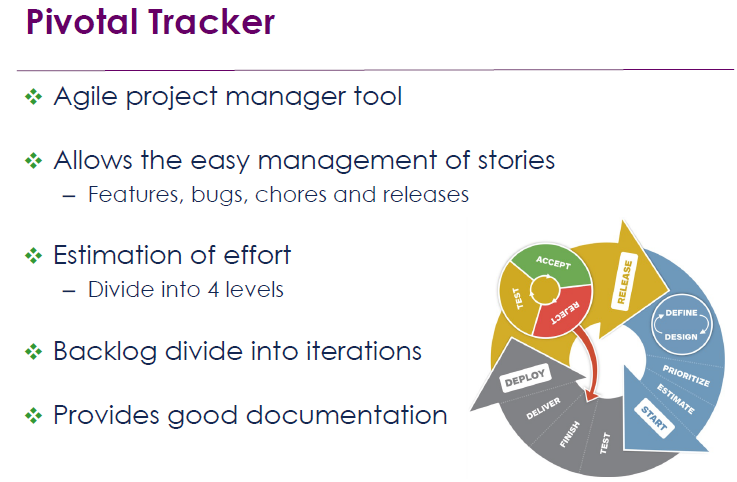
\includegraphics[scale=0.6]{47}
\end{center}

\subsubsection*{Workflow Overview}

\begin{enumerate}
  \item Escrever stories;
  \item Priorizar stories;
  \item Estimar stories;
  \item Começar stories;
  \item Acabar e entregar stories;
  \item Testar stories;
  \item Aceitar ou rejeitar stories;
  \item As stories vão para o painel de "Done";
\end{enumerate}

\subsubsection*{GitHub}

\begin{itemize}
  \item É mais do que um repositório de código;
  \item Tem funcionalidades de gestão de projetos
  \begin{itemize}
    \item Gestão de equipas;
    \item Track de issues (podem seguir principios semelhantes a stories);
  \end{itemize}
  \item A comunidade cria novas apps de forma continua (para gestão personalizada);
\end{itemize}

\subsubsection*{GitHub Marketplace}

Apps para integrar nos GitHub projects. Possiu diferentes categorias:
Code review, continuous integration, security, testing, monitoring, \dots

\pagebreak

\subsubsection{Design e Implementação}

Feature-branching workflow, com repositórios de código,
utilizando Git como sistema de controlo de versões.

\begin{center}
  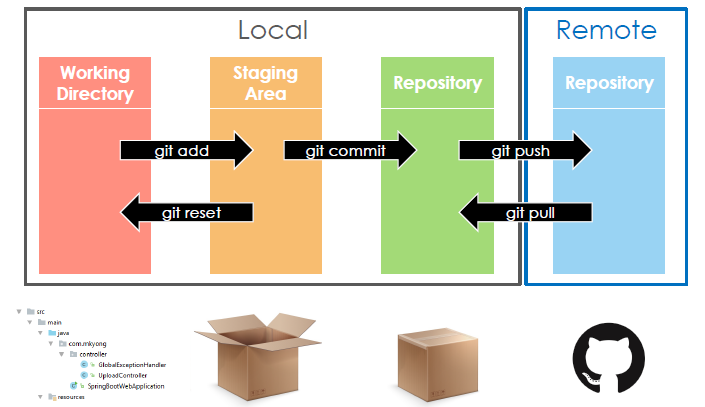
\includegraphics[scale=0.6]{48}
\end{center}

\subsubsection*{O que é um commit?}

É uma operação fundamental para gravar mudanças no repositório.
Um hash SHA-1 único é utilizado para identificar o commit.

\vspace{2mm}

\textbf{Inclui}: O conteúdo do ficheiro commited, a mensagem de commit, o
nome e email do autor, o nome e email do commiter, timestamp
e talvez mais\dots

\subsubsection*{Commits diários}

\begin{flushleft}
  \textbf{Cenário}
  \begin{itemize}
    \item Trabalhar num projeto por duas semanas sem fazer um único commit;
    \item O disco do computador decide morrer;
    \item \textbf{E agora?}
  \end{itemize}

  Nunca se deve esperar que uma funcionalidade esteja completa
  para fazer um commit. \textbf{Todos os dias}, deve-se fazer
  \uline{commit} do trabaho e \uline{push} ao código para o repositório.
\end{flushleft}

\pagebreak

\subsubsection*{Git Workflow}

\begin{center}
  \includegraphics[scale=0.6]{49}
\end{center}

\subsubsection*{Nova release}

 \begin{itemize}
  \item Preparar o produto para ser mostrado ao cliente, Fachando assim
  um ciclo de desenvolvimento;
  \item Checkout de um dev;
  \item Quando a release está pronta: merge à release para a master e
  merge da branch para o dev;
 \end{itemize}

 \begin{center}
  \includegraphics[scale=0.6]{50}
 \end{center}

\pagebreak

\subsubsection*{Hotfix}

\begin{itemize}
  \item Um bug catastrófico foi encontrado;
  \item O que fazer?
  \begin{itemize}
    \item Checkout da master;
    \item Corrigir o bug;
    \item Merge para a master e a dev;
  \end{itemize}
  \item Normalmente não é preciso uma nova branch para uma release;
\end{itemize}

\begin{center}
  \includegraphics[scale=0.6]{51}
\end{center}

\subsubsection*{Nova feature}

\begin{itemize}
  \item \textbf{Nova branch} para cada feature;
  \item Checkout da dev;
  \item Quando a feature está completa: merge da dev para a feature,
  merge da branch para a dev;
\end{itemize}

\begin{center}
  \includegraphics[scale=0.6]{52}
\end{center}

\subsubsection*{Pull/Merge Requests}

\begin{itemize}
  \item Dar merge a branches precisa de um pedido, normalmente para
  proteger as branches (master e dev);
  \item Um pull request precisa de aprovação, normalmente do manager
  do git (DevOps Master);
  \item Por vezes a implementação precisa de melhorias, como quando uma
  feature não está completa ou conflitos complexos durante o merge;
\end{itemize}

\pagebreak

\subsubsection{Merge Workflow}

\begin{itemize}
  \item Commit interlock (lock de commits);
  \item Dificil de seguir o histórico de commits;
\end{itemize}

\begin{center}
  \includegraphics[scale=0.6]{53}
\end{center}

\subsubsection{Rebase Workflow}

\begin{itemize}
  \item Não há interlock de commits;
  \item É mais fácil de comunicar o histórico de commits;
\end{itemize}

\begin{center}
  \includegraphics[scale=0.6]{54}
\end{center}

\subsubsection{Merge ou Rebase?}

\begin{flushleft}
  \textbf{Merge}
  \begin{itemize}
    \item \textbf{Vantagens:} Non-destructive, branches existentes não são
    alterados de qualquer maneira, apenas temos um novo commit (fácil de reverter);
    \item \textbf{Desvantagens:} Polui o histórico do repositório, torna dificil
    de perceber a evolução;
  \end{itemize}

  \textbf{Rebase}
  \begin{itemize}
    \item \textbf{Vantagens:} Projeto muito mais limpo, com histórico do projeto linear;
    \item \textbf{Desvantagens:} Fácil de fazer mal, reescrevendo o histórico, mais dificil de resolver conflitos;
  \end{itemize}
\end{flushleft}

\pagebreak

\subsubsection{Nomes das Branches}

Cada programador gosta da sua própria convenção, no entanto estas convenções não
são standards. O nome das branches é importante, como nomes bons para
variáveis no código.

\begin{center}
  \includegraphics[scale=0.6]{55}
\end{center}

Por exemplo um URL dá redirect para a página errada, \#123:
\begin{itemize}
  \item bug/fixURLRedirect (bom)
  \item bug/fix\_url\_redirect (também é bom)
  \item bug/fix\_url\_redirect\_123 (melhor)
\end{itemize}

Se for para a página errada do perfil: bug/accounts/fix\_url\_redirect\_123

\subsection{Troubleshooting}

Dar merge a conflitos que são muito complexos:
\begin{itemize}
  \item Pedir ao developer para dar update à branch;
  \item Dar merge à dev atual para a branch;
\end{itemize}

\vspace{2mm}

Se dermos commit a dados sensíveis, é possível reverter mas pode ser perigoso.

\vspace{2mm}

Dependências: "It works on my machine".

\subsection{Desenvolvimento baseado em contentores}

\begin{itemize}
  \item Uma boa solução para problemas de dependências;
  \item Todos utilizam o mesmo ambiente;
  \item Ambientes de produção e desenvolvimento são muito semelhantes;
  \item Simplifica a integridade de diferentes serviços;
  \item Fácil de dar deploy;
\end{itemize}

\pagebreak

\subsubsection{Virtualização e Containerização}

\begin{center}
  \includegraphics[scale=0.6]{56}
\end{center}

\subsubsection{Docker}

As imagens de produção e desenvolvimento são as mesmas, apenas possuem diferentes
configurações. Em produção:
\begin{itemize}
  \item Utiliza-se \textbf{sempre} volumes para dados sensíveis;
  \item Os containers morrem, mas os volumes não (normalmente);
\end{itemize}

\subsubsection{Imagens}

\begin{itemize}
  \item As imagens são baseadas em contentores;
  \item Uma imagem pode servir múltiplos contentores, mas um contentor
  só pode ser uma imagem;
  \item Permite herança:
  \begin{itemize}
    \item FROM ubuntu:20.04
    \item FROM myImage:base
  \end{itemize}
\end{itemize}

\subsubsection{Docker Compose}

\begin{itemize}
  \item Simplifica a integração entre contentores;
  \item Permite a orquestração de contentores, baseada numa certa ordem;
  \item Não devemos alterar o ficheiro docker-compose.yml
  \begin{itemize}
    \item Em vez disso, devemos definir variavéis (.env);
    \item Criar um ficheiro .env-example com as variavéis base;
  \end{itemize}

  \item Depois de toda a configuração, o startup é trivial: \textbf{docker-compose up -d}
\end{itemize}

\uline{Exemplo nos slides 45-54}

\pagebreak

\section{Padrões de Arquitetura Enterprise}

A \textbf{Arquitetura} é o \textbf{conceito de mais alto nível} para
os desenvolvedores experientes. Define-se como um \uline{Conhecimento
partilhado} que descreve como o \textbf{sistema se divide em componentes}
e como é que estes interagem entre si através de \uline{interfaces}.

\begin{flushleft}
  \textbf{Nota:} Diz-se \textbf{conhecimento partilhado} porque todos o
  desenvolvedores do projeto devem ter noção da arquitetura.

  Cada componente mais abstrato é composto por vários componentes mais
  pequenos, mas se estes não forem do conhecimento/compreensão de todos os desenvolvedores,
  então não fazem parte da arquitetura.
\end{flushleft}

\subsection{Decisões de Arquitetura}

As \textbf{decisões arquiteturais} têm um \uline{grande impacto} na estrutura do projeto, pelo que implicam
decisões bem pensadas e que nem sempre são fáceis de tomar.

\vspace{2mm}

Por exemplo, a decisão de desenvolver uma user interface \textbf{web-based}
para a aplicação, ou a decisão de usar as java server  faces (JSF)
como a \textbf{web framework}. A decisão em que os componentes devem estar
\textbf{distribuídos} remotamente para uma maior escalabilidade, ou
a decisão de usar \uline{REST} para \textbf{comunicar} entre componentes
distribuidos.

\vspace{2mm}

Por isso, embora quando tomadas possam parecer demasiado óbvias e irrelevantes, \textbf{devem ser
bem documentadas}, identificando as condições e restrições e analizando cada opção com
base nas anteriores.

\vspace{2mm}

Caso contrário, pode acontecer o anti-pattern \textbf{Groundhog Day}, que
diz que \uline{decisões arquiteturais importantes} que foram feitas
são perdidas, esquecidas ou não são comunicadas de forma eficiente.
Ninguém percebe \uline{o porquê da decisão ter sido feita}, continuando
a ser discutida outra e outra e outra vez\dots


\subsubsection{Justificar Decisões}

\begin{enumerate}
  \item Identificar as condições e restrições;
  \item Analisar cada opção com base nas condições;
  \item Tomar uma decisão;
  \item Justificar a decisão;
\end{enumerate}

\subsection{Documentação e Comunicação}

Desde cedo estabelecer onde as decisões arquiteturais serão documentadas
e \textbf{ter a certeza que todos os membros da equipa sabem} onde
ir para encontrar a informação. Num documento ou wiki, em vez de ter
múltiplos ficheiros espalhados por uma drive partilhada que já tem
muitos ficheiros. A documentação deve ser \textbf{centralizada}.

\vspace{2mm}

Soluções email-driven (horrível): as pessoas esquecem-se, perdem,
ou não sabem que uma decisão de arquitetura foi tomada, logo, não implementam
a arquitetura corretamente.

\pagebreak

\subsection{Evitar a Arquitetura \uline{Witches Brew}}

As arquiteturas desenhadas por grupos resultam em ideias complexas
todas misturadas e sem visão clara. O problema começa quando
os membros da equipa começam a discutir ideias completamente
diferentes, e a baralhar tudo.

\vspace{2mm}

É fundamental que a equipa recolha o melhor do \textbf{conhecimento coletivo} de forma a atingir uma
solução comum e consensual, chegando a uma \uline{visão unificada
para a arquitetura}. A arquitetura não deve por isso sem feita em pequenos grupos
dentro da equipa, podendo nestes casos levar a uma mistura complexa de ideias sem uma
visão clara do que deve efetivamente ser implementado.


\subsection{Padrões de Arquitetura de Software}

\subsubsection{Os mais simples}

 \begin{flushleft}
  \textbf{Cliente-Servidor} - Esta arquitetura consiste na relação
  de um para um entre o cliente e o servidor (ex: aplicações online, email).

  \begin{center}
    \includegraphics[scale=0.6]{57}
  \end{center}

  \textbf{Master-Slave} - Semelhante à anterior no que toca ao número de
  intervenientes na relação, mas distinta porque no servidor há um relacionamento
  interno de um para muitos, master/slave. Por exemplo:
  aplicações multi-threaded ou relplicações de bases de dados.

  \begin{center}
    \includegraphics[scale=0.6]{58}
  \end{center}

  \textbf{Pipe-filter} - É utilizada em processos que exisgem buffering
  (começamos numa fonte de dados e acabamos num consumidor de dados, podendo utilizar
  filtros pelo meio) ou sincronismo. Por exemplo: compiladores,
  processos em cascata (streamed), buffering ou sync.

  \begin{center}
    \includegraphics[scale=0.6]{59}
  \end{center}
 \end{flushleft}

\pagebreak

\subsubsection{Arquitetura Microkernel}

Tem por base dois componentes: a \textbf{core} application/system (estável) e os \textbf{plugins} (dinâmicos).
Novas funcionalidades da aplicação são adicionadas como plugins, que são
independentes do core, fornecendo extensibilidade, flexibilidade e
isolamento e separação de funcionalidades da lógica da aplicação.

\begin{center}
  \includegraphics[scale=0.7]{60}
\end{center}

O \textbf{core system} geralmente providencia apenas as funcionalidades básicas
e estritamente necessárias ao funcionamento do sistema. Deve ainda ter conhecimento
dos plugins disponíveis e de como os obter (nome, contratos e protocolos de acesso).
Pode ser integrado ou como parte de outro padrão de arquitetura. É uma boa
primeira escolha para aplicações baseadas em produtos.

\vspace{2mm}

\begin{flushleft}
  \textbf{Exemplo:} Os IDE fornecem um core system que depois é complementado
  pelos plugins que lhe adicionam novas funcionalidades.
\end{flushleft}

\subsubsection{Arquitetura em camadas (Layered Architecture) (n-tier)}

Este é o padrão arquitetural mais comum hoje em dia (standard para a
maior parte das aplicações Java EE). Os seus componentes são baseados em
camadas horizontais, cada uma com um papel específico na aplicação
(separation of concerns).

\begin{center}
  \includegraphics[scale=0.55]{61}
\end{center}

A sua característica principal é a \textbf{separação de papéis} que cada camada
desempenha, sendo este específico para cada uma, que lida apenas com a lógica adjacente a si mesma.
Cada camada forma assim uma camada de \textbf{abstração}.

É muito semelhante à organização estrutural encontrada em muitas
empresas. É um padrão general-purpose sólido, fazendo com que seja
um bom ponto de partida para a maioria das aplicações.

\vspace{2mm}

\begin{flushleft}
  \textbf{Exemplo:} A camada de apresentação não precisa de saber como obter
  os dados do user, tendo como única preocupação a forma como os vai apresentar,
  a única lógica que implementa.
\end{flushleft}

\pagebreak

\subsubsection{Arquitetura Event-Driven}

Consiste num padrão de arquitetura \textbf{distribuida e assincrona}
utilizado para cirar \uline{aplicações escaláveis}, também conhecido por
\textbf{message-driven} ou \textbf{stream processing}. É composto por
componentes individuais desacoplados que recebem e processam eventos
assincronamente.

\begin{center}
  \includegraphics[scale=0.55]{62}
\end{center}

Este padrão é relativamente \textbf{complexo} de implementar, principalmente
devido à sua natureza assincrona distribuida. \textbf{Falta de transações
atomicas} para apenas um proceso de negócio:
\begin{itemize}
  \item Os componentes do processamento de componentes são altamente
  desacoplados e distribuidos;
  \item É muito dificil de manter uma unidade transacional de trabalho
  através de todos os componentes;
\end{itemize}

Um aspeto chave é a \textbf{criação, manutenção e governação} dos contratos
dos componentes processadores de eventos. Útil em eventos com
várias etapars e que necessitam de orquestração para serem processados.

\vspace{2mm}

\begin{flushleft}
  \textbf{Exemplo:} Suponhamos que uma pessoa muda de casa e informa a sua
  seguradora, através de um evento relocation. Os passos envolvidos no seu processamento estão contidos num event
  broker, como mostrado na figura acima, que por cada passo vai criar um processing event, que é depois enviado
  para o canal correspondente, onde será processado pelo seu event consumer. O processo continua até que todos os
  passos estejam concluídos.
\end{flushleft}

\subsubsection{Arquitetura Orientada a Serviços (SOA)}

\begin{center}
  \includegraphics[scale=0.55]{63}
\end{center}

\pagebreak

Esta arquitetura tem como objetivo desenvolver serviços distribuídos cujos
componentes são serviços standalone e podem ser utilizados por outros
como serviços prontos a consumir (não como bibliotecas).

\begin{center}
  \includegraphics[scale=0.55]{64}
\end{center}

As características chave deste tipo de arquitetura são: \textbf{contratos standardizados de serviços},
\textbf{independente da linguagem}, \textbf{baixo acoplamento}, \textbf{reutilização}
e \textbf{autonomia}.

\vspace{2mm}

\begin{flushleft}
  \textbf{Exemplo:} Na UA o sistema de autenticação é utilizado por todos os serviços associados ao ensino. Foi desenvolvido
  como um componente standalone e é utilizado por outros serviços como um serviço (neste caso de auntenticação)
  como o PACO, o Elearning, o site do NEI\dots
\end{flushleft}

POde ainda ser adicionada uma camada de \textbf{abstração} quando
há vários componentes para o mesmo serviço com um servige registry.
Este é contactado pelo cliente para saber qual componente está disponível.

\begin{flushleft}
  \textbf{Exemplo:} Na  UA podiam existir vários sistemas de impressão que trabalhavam de forma complementar para
  aumentar a redundância. Quando queríamos imprimir contactavamos o registo dos serviços que nos dizia qual o
  sistema que estava disponível, para o qual era enviado o pedido de impresão.  
\end{flushleft}

\subsubsection*{SOAP (Simple Object Access Protocol)}

Este é um protocolo baseado em XML que foi pioneiro na definição de comunicação
entre aplicações, independentemente da plataforma linguagem de programação em que
são desenvolvidos.

\textbf{Serviços Web baseados em SOAP/WSDL:} Por ser uma solução muito abrangente e demasiado estandardizada
(tem estrutura pré-definida) foi considerada demasiado pesada e
pouco eficiente.

\begin{center}
  \includegraphics[scale=0.38]{65}
\end{center}

\pagebreak

\subsubsection*{REST (Representational State Transfer)}

Para simplificar as comunicações foi criado o REST, que com menos
estandardização torna a \uline{comunicação entre processos mais simples}.
É um estilo arquitetural baseado na \textbf{transferência de representações
de recursos} de um servidor para um cliente. É \textbf{bem mais simples}
do que SOAP/WSDL para implementadar serviços web.

Os serviços RESTful involvem uma carga (overhead) mais pequena do que
as chamadas "big web services".

\vspace{2mm}

Tem por base a utilização de \textbf{endpoints HTTP}, através de pedidos
GET, POST, DELETE, PUT, através dos quais são trocadas mensagens em formato
JSON. Fornece uma forma de comunicação sem estado, mais simples e
mais leve.

\vspace{2mm}

Um elemento fundamental nesta arquitetura são os \textbf{recursos}
(catálogo, registo médico ou documentos, \dots) (múltiplas representações,
podendo existir em formatos diferentes (JSON, TXT, \dots)) sobre os quais são feitas as operações CRUD
(Create, Read, Update, Delete).

\begin{center}
  \includegraphics[scale=0.4]{66}
\end{center}

\begin{flushleft}
  \textbf{Nota:} O create é feito pedido pedido POST, o read pelo GET, o update pelo PUT e o delete pelo DELETE.
\end{flushleft}

Aprensenta no entanto algumas desvantagens, nomeadamente a
\textbf{dificuldade em representar recursos/interfaces complexas},
a \textbf{necessidade de documentar} as interfacees para as entender, uma vez que não
existe descrição standard, e ainda a \textbf{necessidade de implementar
sistemas adicionais} para monitorizar e gerir a qualidade de
um serviço e a fiabilidade do serviço (ex: REST não
coloca qualuqer tipo de segurança como o SOAP).

\subsubsection*{Topologia SOA}

Esta arquitetura era inicialmente para desenvolver aplicações
monolíticas, mas evoluiu a partir de então. Muitas organizações
utilizam o SOA para resolver complexidades de integração, através
de \textbf{Enterprise Service Bus (ESB)} (middleware de mensagens).

\pagebreak

\begin{center}
  \includegraphics[scale=0.4]{67}
  \includegraphics[scale=0.4]{68}
\end{center}

Algumas caracteríscas chave do \textbf{ESB} são:
desenvolvimento streamlined, suporta várias estratégias de binding,
realiza várias trasformações dos dados, routing inteligente, monitorização em
tempo real, tratamento de exceções e serviço de segurança.

\subsubsection{Arquitetura de Microserviços}

Este padrão evoluiu de \textbf{2 fontes principais}:
\begin{itemize}
  \item aplicações desenvolvidas ustilizadno o padrão por camadas;
  \item aplicações distribuidas desenvolvidas utilizando uma arquitetura orientada a serviços (SOA);
\end{itemize}
Procura simplificar o seu desenvolvimento através da sua divisão em pequenos serviços.

\vspace{2mm}

O principal conceito deste padrão é a noção de \textbf{deploy de unidades
separadas}. Estas unidades são componentes que prestam um serviço (deployed
como uma unidade separada) e
podem consistir num pequeno módulo ou numa grande porção da
aplicação. Permitem uma deployment mais fácil e desacoplamento.

\vspace{2mm}

Em qualquer um dos cenários deve ser assegurada uma \textbf{arquitetura
distribuída}, para a qual é fundamental o desacoplamento total entre os
componentes e a definição do seu protocolo de acesso (REST, SOAP, JMS,
…). \uline{O grande desafio é atingir o grau certo de granularidade}.

\begin{flushleft}
  \textbf{Nota:} Se for necessário orquestrar ou passar mensagens entre os componentes na camada da interface ou API, então o
  serviço está demasido granulado. Caso esta não consiga ser reduzida (ou seja, por mais que tentemos a orquestração
  não deixa de ser necessária), então este não será o padrão adequado para desenvolver a nossa aplicação.
\end{flushleft}

\begin{center}
  \includegraphics[scale=0.5]{69}
\end{center}

As aplicações são geralmente \uline{mais robustas}, \uline{fornece melhor escalabilidade}, e \uline{pode
suportar mais facilmente a entrega continua}. A capacidade de realizar
deployments de produção em real-time. Apenas os componentes do serviço
que mudam precisam de ser deployed.


\pagebreak


\subsubsection*{SOA vs Microservices}

\begin{center}
  \includegraphics[scale=0.5]{70}
\end{center}

\subsubsection{Arquitetura Space-Based}

A maioria das aplicações web gere os pedidos num Fluxo
servidor $\rightarrow$ aplicação $\rightarrow$ base de dados,
fornecendo uma resposta em tempo útil para um fluxo notmal de acesso.
No entanto, quando \uline{o fluxo começa a crescer começamos a assistir
a um aumento do contrangimento do tráfego}. Inicialmente no servidor, que pode ser expandido facilmente e
sem grandes custos, mas que faz com que se comecem a sentir limitações na aplicação, esta
mais difícil e cara para expandir e por fim na base de dados, que também requere um grande
investimento para a sua expansão.

\vspace{2mm}

A \textbf{space-based architecture}, também conhecido por \textbf{cloud architecture} procura então resolver
os problemas de \textbf{escalabilidade e concorrência}, consistindo numa melhor alternativa à de tentar
escalar os elementos do referido fluxo. É uma boa escolha para aplicações
com load variavel (ex: redes sociais, sites de leilão, \dots).

\begin{center}
  \includegraphics[scale=0.5]{71}
\end{center}

O nome deste padrão vem do conceito de \textbf{tuple space}, um paradigma de memória partilhada
distribuída que implementa através da remoção da base de dados central, criando uma rede
de dados replicada em memória.

\vspace{2mm}

Cada \textbf{unidade de processamento} vai então ter uma cópia da base de dados, pelo que estas
podem ser inicializadas e desligadas dinâmicamente de acordo com a variação do tráfego de
acesso.

\pagebreak

\section{Web Frameworks - Spring}

Até há uns anos atrás, os programas corriam apenas localmente nos computadores.
Hoje em dia é muito diferente, as aplicações web têm um papel central nas
aplicações que utilizamos diariamente.

\vspace{2mm}

As páginas web evoluiram de versões \textbf{estáticas}, que
retornam conteúdos hardcoded armazenado no servidor quando um
recurso particular é requisitado.

\begin{center}
  \includegraphics[scale=0.45]{72}
\end{center}

Nas \textbf{dinâmicas}, o conteúdo das páginas é gerado dinamicamente,
apenas quando necessário, normalmente introduzindo informação de bases
de dados em templates HTML.

\begin{center}
  \includegraphics[scale=0.45]{73}
\end{center}

Um site dinâmico pode retornar dados diferentes para um URL,
baseado na informação fornecida pelo user ou preferências
armazenadas e pode realizar outras operações como parte de
retornar uma resposta (ex:  mandar notificações).

\vspace{2mm}

A maior parte do código que suporta o website dinâmico corre num servidor
web. Criar este código é conhecido como \textbf{server-side} programming
ou \textbf{backend} programming.

\vspace{2mm}

Para que serve o \textbf{backend}? Como sabemos, os programas executam
código binário, e também texto (linguagens interpretadas),
mas o browser não consegue entender binário, apenas HTML
e alguns outros scripts (ex: JavaScript). O backend
terá como função gerar (ou obter de uma base de dados) dados
e enviar para o clent-side (browser) em HTML.

\subsection{Frameworks}

Nos anos 2000 começaram a surgir finalmente as frameworks, que quer sejam focadas no lado
do servidor ou do cliente, são um \textbf{design reutilizável} de todas
as partes do sistema que é representado por um conjunto de classes
abstratas e na forma que as suas intâncias interagem (estrutura).
Fornecem um \textbf{esqueleto} de uma aplicação, que pode ser
\textbf{customizado} pelo programador.

\pagebreak

\begin{flushleft}
  \textbf{Exemplo:} A framework \textbf{Spring} permite gerar o esqueleto
  para um projeto Maven e com alguns cliques no Spring Initializr ter
  uma aplicação a dar Hello World sem ter de escrever qualquer linha de código.

  Desta forma evita a "reinvenção da roda", evitando a escrita  do código comum
  a vários proejtos cada vez que se cria um novo.
\end{flushleft}

Uma framework fornece uma fundação de software genérica, sobre a qual
\textbf{código personalizado específico par a aplicação} pode ser secrito.
Normalmente incluem múltiplas bibliotecas, juntamente com ferramentas e
regras de como estruturar e usar os componentes.

\vspace{2mm}

As frameworks diferem de classes de outras bibliotecas através da reutilização
do design de alto nível.
\begin{itemize}
  \item \textbf{As bibliotecas são usadas pelo código especifico
  da aplicação} para suportar funcionalidades específicas;
  \item \textbf{As frameworks controlam o flow da aplicação}
  e chamam o código específico da aplicação;
\end{itemize}

\subsubsection*{Frameworks e Bibliotecas}

\begin{flushleft}
  \textbf{Bibliotecas:} Chamam as funções na API para fazerem coisas por nós;

  \vspace{2mm}

  \textbf{Frameworks:} "Don't call us, we'll call you", containers
  de inversão de controlo;
\end{flushleft}

\begin{center}
  \includegraphics[scale=0.6]{74}
\end{center}

\subsubsection{Vantagens}

\begin{itemize}
  \item Poderosas e complexas;
  \item Velocidade de implementação;
  \item Soluções testadas e comprovadas;
  \item Acesso a soluções off-the-shelf;
  \item Manutenção (updates,\dots);
\end{itemize}

\subsubsection{Desvantagens}

\begin{itemize}
  \item Dificil de aprender;
  \item Performance mais baixa;
  \item Independência reduzida;
  \item Dependência de entidades externas;
  \item Lock-in tecnológico;
\end{itemize}

\pagebreak

\subsection{Client-Side Frameworks (Frontend)}

As mais utilizadas são o \textbf{Angular}, \textbf{React} e \textbf{Vue.js} e permitem vérias funcionalidades.
\begin{itemize}
  \item \textbf{Manipulação de documentos} carregados pelo browser -
  O DOM (Document Object Model) permite a manipulação de um documento junto com HTML e CSS;

  \item \textbf{Atualizar dados (Fetch)} - Através de chamadas assíncronas ao
  servidor (ex: AJAX);

  \item \textbf{Desenhando e manipulando gráficos} - complexo com desenho no navegador;
  \item \textbf{Armazenamento Client-Side} - através de "bases de dados" locais
  (ex: IndexedDB)
\end{itemize}

\subsection{Server-Side Frameworks (Backend)}

\begin{flushleft}
  \textbf{Componentes Core:}
  \begin{itemize}
    \item \textbf{Request Routing} - Faz a ligação entre os HTTP requests e o código;
    \item \textbf{Data Access} - Acesso a dados uniforme, mapeamento e configuração;
    \item \textbf{Template Engine} - Estruturar e separar a apresentação da lógica; 
  \end{itemize}

  \textbf{Componentes Comuns:}
  \begin{itemize}
    \item \textbf{Security} - Proteção contra ataques web comuns;
    \item \textbf{Sessions} - GEstão de sessões e configurações;
    \item \textbf{Error Handling} - Capturar e gerir erros ao nível da aplicação;
    \item \textbf{Scaffolding} - Gerar interfaces de CRUD rapidamente, baseadas em
    modelos de dados;
  \end{itemize}

  \textbf{Por exemplo, em SpringBoot, O Request Routing é feito utilizando
  RequestMapping}
\end{flushleft}

\subsubsection{Acesso aos Dados}

\begin{flushleft}
  \textbf{Independência Lógica:} A habilidade de alterar o esquema lógico sem
  alterar o esquema externo ou programmas de aplicação
  \begin{itemize}
    \item Pode adicionar novos campos, novas tabelas, sem alterar as views;
    \item Pode alterar estruturas de tabeas sem alterar as views;
  \end{itemize}

  \textbf{Independência Física:} A habilidade de alterar o esquema físico
  sem alterar o esquema lógico
  \begin{itemize}
    \item O tamanho do armazenamento pode mudar;
    \item O tipo de alguns dados pode mudar para razões de otimização;
  \end{itemize}

  \textbf{Solução:} Manter a \textbf{VIEW} (o que o user vê) independente do
  \textbf{MODEL} (domínio do conhecimento).
\end{flushleft}

\pagebreak

\subsubsection*{Model-View-Controller (MVC)}

Muitas frameworks de backend seguem, ou são uma evolução de um padrão de
design chamado \textbf{Model-View-Controller (MVC)}.
\begin{itemize}
  \item Separa a funcionalidade core da apresentação  e controlo da lógica
  que utiliza esta funcionalidade;
  \item Permite que múltiplas views partilhem o mesmo modelo de dados;
  \item Torna suportar múltiplos clientes mais fácil de implementar, testar
  e manter; 
\end{itemize}

\begin{center}
  \includegraphics[scale=0.7]{75}
\end{center}

\begin{flushleft}
  \textbf{Model:} Representação por parte do programa do objeto/base de dados (Users, Products, Cars,\dots);
  
  \textbf{View:} A representação visual dos dados. É aquilo que o user
  da web app vê (HTML, CSS, JavaScript);

  \textbf{Controller:} É o go-between entre o Model e a View.
  \begin{itemize}
    \item One way: pega no input da View e dá a ao Model
    para este poder agir;
    \item Other way: Vai buscar os dados dos Model(s) e dá os à View
    para incorporar na representação visual;
    \item \textbf{Exemplo:} Novo signup de um user, listas de produtos
    que são menos do que 10€, redireciona o user.
  \end{itemize}

  \subsubsection{Template Engine}

  As Template Engines pegam nas strings tokenizadas e produzem
  rendered strings com valores nos locais do token como output.
  Estes templates são tipicamente usados como um formato imediato por
  desenvolvedores para, programaticamente, produzir um ou mais
  output formats desejados. Normalmente, HTML, XML ou PDF (ex:
  Java Server Pages, Thymeleaf).
\end{flushleft}

\pagebreak

\subsection{Spring Framework}

\begin{itemize}
  \item Arquitetura
  \item Anotações
  \item Inversion of Control (IoC)
  \item Dependency Injection (DI)
  \item Beans
  \item Aspect-Oriented Programming (AOP)
\end{itemize}

Spring não foi a primeira framework a tentar resolver os problemas
relacionados com a contrução de aplicações empresariais em Java.
\textbf{J2EE ou Java EE (Enterprise Edition)} que deu origem
ao Spring tentou fazer a mesma coisa, fornece uma boa separação
entre várias partes da aplicação.

No ínicio dos anos 2000, surgiu a \textbf{Spring Framework},
desde então, cresceu de ser um (já sofisticado) \uline{cointainer de
injeção de dependências} para um \textbf{ecosistema de frameworks
que cobre vários casos de uso} no desenvolvimento de uma aplicação.

Coexiste com a \textbf{JEE} (Java Enterprise Edition), mais tarde \textbf{Jakarta EE}. Apesar de definirem
especificações distintas, a Spring implementa algumas do EE.

\begin{flushleft}
  \textbf{Nota:} Para cada interface o JEE define \textbf{JSR} -
  Java Specification Request, que estabelecem a interface para cada
  funcionalidade.
\end{flushleft}


\subsubsection{Arquitetura}

\begin{center}
  \includegraphics[scale=0.35]{76}
\end{center}

A arquitetura Spring divide-se em vários componentes como podemos verificar.


\pagebreak

O \textbf{core container} tem quatro múdulos, que são a base de qualquer
aplicação:
\begin{itemize}
  \item \textbf{Spring Core} - Fornece implementação para funcionalidades
  como IoC (Inversion of Control) e DI (Dependency Injection);
  \item \textbf{Spring Beans} - Este módilo fornece implementações do padrão de fábrica
  do BeanFactory;
  \item \textbf{Spring Context} - Contrói em cima do Core e Beans e fornece
  uma forma de aceder a objetos definidos e fornece suporte a interações
  third-party como caching, mailing, and template engines. A interface ApplicationContext é a
  a core part deste módulo;
  \item \textbf{Spring Expression Language (SpEL)} - Permite aos utilizadores
  usarem a String Expression Language para aceder e manipular o gráfo de
  objetos durante a runtime;
\end{itemize}

\subsubsection{Anotações}

No processo de compilação de um programa é feita uma análise sintática para verificar que o
código cumpre com uma determinada estrutura. No entanto, há situações em que queremos
adicionar verificações adicionais, ou mesmo alterar o código de forma sistemática em
determinados trechos durante o processo de compilação.

\vspace{2mm}

Para reposnder a estes cenários e de forma a evitar a complexidade da
alteração ao código, \uline{metadados que dão informação} sobre o código ao compilador
e que podem ser considerados por outro desenvolvido por nós para esse fim.

Facilita a deteção de erros ou supressão de avisos, por exemplo. Podem
ter informação para o compilador (detetar erros e suprimir warnings),
processamento compile-timee deployment-time, e processamento runtime.
\textbf{As Anotações são muito utilizadas em na Spring Frameworks}.

\begin{flushleft}
  \textbf{Exemplos:}  De anotações interpretadas pelo Java Compiler são o @Override, @Deprecated.

  Caso num programa utilizemos um método de uma classe anotado como @Deprecated, quando compilarmos estes
  programa o compilador irá mostrar-nos o aviso de que estamos a utilizar um método obsoleto.
\end{flushleft}


\subsubsection{Inversão de Controlo (IoC)}

Quando trabalhamos com uma framework, como esta fornece a maioria das funcionalidades
necessárias ao funcionamento de uma aplicação web, a framework passa a ser a responsável
pela \textbf{criação dos objetos}.

IoC é um processo em que definimos uma classe, mas não criamos
os objetos (apenas definimos como devem ser criados pelo
IoC container).

\begin{center}
  \includegraphics[scale=0.4]{77}
\end{center}

O atributo \uline{name} da propriedade no XML deve ser mapeado getName e setName
na classe do objeto a criar com \uline{Name} o valor de outro atributo.

No exemplo acima para o atributos id e name devem haver os métodos getId() e setId() e getName() e setName().

\subsubsection{Injeção de Dependências (DI)}

Quando um objeto tem como atributo outro objeto, vai depender dele, sendo por isso
necessário criá-lo antes do primeiro. A \textbf{injeção de dependências}
é um padrão que \uline{remove as dependências dp código}.
Podemos especificar as dependendências das classes através de
\textbf{anotações} ou ficheiros externos como um XML.

A injeção pode ser através de um contrutor ou de um seller.

\subsubsection*{POJO (Plain Old Java Object)}

\begin{center}
  \includegraphics[scale=0.4]{78}
\end{center}

\subsubsection*{Com Spring DI}

\begin{center}
  \includegraphics[scale=0.4]{79}
\end{center}

Em \textbf{Spring} as classes identificadas com a anotação @Component são geridas de
acordo com estes princípios de IoC e DI pelo \textbf{Spring Container}.
O Spring IoC é o coração da Spring Framework, cada objeto delega o \textbf{trabalho
de contruir} um IoC container. Este recebe metadados a partir de ficheiros XML,
anotações Java ou código Java e produz um sistema ou uma aplicação completamente
configurado e pronto a correr.

\begin{center}
  \includegraphics[scale=0.4]{80}
\end{center}

As principais tarefas realizadas pelo IoC container são:
\begin{itemize} 
  \item Instanciar o bean/objeto;
  \item Escrever os beans juntos (injeção de dependências estre eles);
  \item Configurar os beans;
  \item Gerir o ciclo de vida dos beans;
\end{itemize}

Existem dois tipos de Spring IoC containers (interfaces):
\begin{itemize}
  \item \textbf{BeanFactory} - É o container mais simples, fornece
  a configuração da framework e funcionalidades básicas;
  \item \textbf{ApplicationContext} - contruído em cima da interface
  BeanFactory, adiciona mais funcionalidades enterprise-specific (várias
  interfaces para implementações distintas);
\end{itemize}

\pagebreak

\subsubsection{Beans}

São definidas pela documentação Spring como os objetos base da aplicação (backbone), que são geridos
pelo Spring IoC Container (desde a instanciação e construção até à gestão).

Algumas características chave dos beans são:
\begin{itemize}
  \item Todos os campos devem ser \textbf{privados};
  \item Todos os campos devem ter \textbf{getters e setters};
  \item Devem ter um \textbf{construtor vazio};
  \item Os campos são acessados exclusivamente através dos getters/setters
  e construtor;
\end{itemize}

O Spring é responsável por criar os objetos bean, mas, primeiro, temos de
dizer à framework quais são os objetos que queremos que sejam criados.
As \textbf{Bean definitions} dizem ao Spring quais classes a framework deve usar
como beans. As Bean definitions são como receitas (também descrevem
as propriedades do bean).

\vspace{2mm}

Existem \textbf{3 formas diferentes} de definir um Spring Bean:
declarar a definição num \textbf{ficheiro XML configurável},
anotando uma classe com a anotação \textbf{@Component} (ou derivadas como
@Service, @Repository, @Controller) ou escrevendo um bean factory method
anotado com a anotação \textbf{@Bean} num class Java personalizada de configuração. 

Hoje em dia apenas se usam os dois últimos, mas o outro ainda é permitido
para compatibilidade com versões anteriores.

A \textbf{escolha entre os métodos de bean definition}
é principalmente ditada pelo acesso ao código fonte da classe que
queremos usar como um Spring Bean.

\vspace{2mm}

A anotação @Component é utilizada quando \textbf{temos acesso ao código fonte}. Quando esta só tem um construtor, o
Spring considera os seus parâmetros como a lista de dependências obrigatórias. Caso haja mais do que um, devemos
anotar o que define as dependências com @Autowired.

No runtime, o Spring vai procurar por classes anotadas com @Component
e vai usá-las como definições de bean. O processo de procurar por
classes anotadas chama-se \textbf{component scanning}.

\vspace{2mm}

Quando \textbf{não temos acesso ao código fonte} da classe, definimos uma classe com um método de fábrica anotado com
@Bean. Esta classe por sua vez é anotada com @Configuration, que marca a classe como sendo um container de
definições @Bean. Podem ser definidos vários métodos de fábrica dentro da mesma classe de configuração.

\begin{center}
  \includegraphics[scale=0.5]{81}
  \includegraphics[scale=0.5]{82}
\end{center}

\subsubsection{Spring Expression Language (SpEL)}

Pode ser usada para manipular e aceder a um gráfo de objetos durante a runtime. SpEL está disponível
via XML ou anotações e é avaliado durante o tempo de criação do bean.

Possuí vários operadores disponíveis como:
\uline{aritméticos} (+, -, *, /, \%), \uline{relacionais} (==, !=, <, >, <=, >=),
\uline{lógicos} (and, or, not), \uline{condicionais} (?:), \uline{regex} (matches).

\pagebreak

\begin{center}
  \includegraphics[scale=0.3]{83}
  \includegraphics[scale=0.3]{84}
\end{center}

A anotação \textbf{@Value} permite a injeção de valores nos atributos nos beans

\subsubsection{Aspect-Oriented Programming (AOP)}

É uma abordagem de programação que permite a propriedades
globais de um programa \textbf{determinarem como é que o código
é compilado} para um programa executável.

É um paradigma complementar à Programação Orientada a Objetos e
que tem como objetivo a separação das responsabilidades de forma
a melhorar a modularidade.

\begin{center}
  \includegraphics[scale=0.5]{85}
\end{center}

AOP \textbf{divide a lógica do programa} em partes distintas chamadas
\textbf{concerns}. Isto aumenta a modularidade através de
\textbf{cross-cutting concerns}. Um \textbf{cross-cutting concern}
é um concern que afeta toda a aplicação e é centralizado
num único local.

AOP pode ser considerado como um padrão de design \textbf{decorador
dinâmico} (o padrão decorador permite que um novo comportamento
seja adicionado a uma classe já existente, dando wrap à classe
original e duplicando a sua interface e depois delegar o origimal).

\subsubsection*{Conceitos AOP Core}

\begin{itemize}
  \item \textbf{Aspect} - Uma modularização de um concern que corta
  múltiplas classes, pode ser uma \textbf{classe} normal,
  cofigurado através de configuração XML ou anotações com @Aspect;
  \item \textbf{JoinPoint} - Um ponto durante a execução do programa,
  onde o fluxo de execução foi alterado devido à exception catching
  ou a chamada de um método;
  \item \textbf{Pointcut} - São basicamente JoinPoints, mas com
  advice (ou call aspect). Expressões que são correspondidas
  em join points para determinar se o advice deve ser executado
  ou não;
  \item \textbf{Advice} - A ação tomada por um aspect num join point
  particular (@Before, @After, @Around, @AfterReturning, @AfterThrowing);
\end{itemize}

\pagebreak

\begin{center}
  \includegraphics[scale=0.35]{86}
\end{center}

\subsubsection{Spring Web}

Este componente aplica a arquitetura Model-View-Controller (MVC).

\vspace{2mm}

Quando recebe um pedido HTTP, o DispatcherServlet consulta o
\textbf{HandlerMapping} para invocar o \textbf{Controller} apropriado.
Este pega mo pedido e encaminha-o para o método adequado de processamento
(GET ou POST) (o método vai dar set ao modelo de dados baseado em
lógica de negógio definida e retorna o nome da view para o DispatcherServlet).

De seguida, o DispatcherServlet pede ajuda ao \textbf{ViewResolver}
para ir buscar a view definida para o pedido. Quando a view wstiver finalizada,
o DispatcherServlet envia o \textbf{modelo de dados para a view}
que é finalmente renderizada no browser.

\begin{center}
  \includegraphics[scale=0.5]{87}
  \includegraphics[scale=0.5]{88}
\end{center}

\pagebreak

\subsubsection{Sprint Data Access Modules}

Há vários módulos que permitem criar a abstração entre os dados e o seu armazenamento.

\begin{flushleft}
  \textbf{JDBC:} Permite trabalhar diretamente com SQL. A camada abstrata
  elimina a necessidade de overhead de exception handling;

  \vspace{2mm}

  \textbf{ORM (Object Relational Mapping):} Ao utilizarmos o ORM temos uma maior abstração, uma vez que trabalhamos sobre objetos Java, sendo
  responsabilidade do módulo mapear as alterações na base de dados.
  Fornece consistência/portabilidade para o código;

  \vspace{2mm}

  \textbf{OXM (Object XML Mapping):} Paradigma de cuma mas sobre XML.
  Converte os objetos para o formato XML e vice-versa. A Spring OXM
  fornece uma API uniforme para acessar qualquer framework OXM;

  \vspace{2mm}

  \textbf{JMS (Java Messaging Service):} Facilita a interação com serviços de
  mensagens. Tem funcionalidades para produzir e consumir mensagens
  entre vários clientes;

  \vspace{2mm}

  \textbf{Transaction:} Facilita a implementação dos conceitos de transações ao nível da organização.
  suporta gestão de transações declarativa e programática para classes que
  implementam interfaces especiais e para todos os POJOs. Todas as transações
  ao nível enterprise podem ser implementadas pelo Spring utilizando este módulo; 
\end{flushleft}

\section{Spring Boot}

Resumidamente, a Spring Framework fornece uma \textbf{infrastrutura
de suporte para o desenvolvimento de aplicações Java}.
Tem muitas funcionalidades, como a Injeção de Dependências e
módulos como o Spring MVC, Spring JDBC, Spring Security,
Spring ORM, Spring AOP, Spring Test.

Estes módulos \textbf{podem reduzir o tempo de desenvolvimento}
de uma aplicação.

\vspace{2mm}

O \textbf{Spring Boot} é uma estensão da Spring Framework, que tem como
objetivo \uline{eliminar a necessidade de definir as configurações padrão}
para iniciar uma aplicação Spring e \uline{fornece uma estrutura
de projeto padrão}, para umdesenvolvimento mais rápido e eficiente.
Algumas funcionalidades são: \uline{"starter" dependencies} para simplificar
a build e as configurações da aplicação, \uline{servidor embutido} para
evitar complexidade e \uline{configurações automáticas para a funcionalidade
Spring}.

\begin{center}
  \includegraphics[scale=0.5]{89}
\end{center}

\pagebreak

Os objetivos principais do Spring Boot são:
\begin{itemize}
  \item \textbf{Redução do tempo de desenvolvimento},
  juntamente com tempo de Unit Test e Integration Test;
  \item Evita completamente a necessidade de \textbf{configuração XML};
  \item Fornece uma \textbf{anotação simples} (baseada nas do Spring);
  \item Evita escrever vários imports;
  \item Abordagem \textbf{opinionated development}, de forma a fornecer
  algumas configurações padrão para começar um novo projeto rapidamente;
\end{itemize}

Os principais componentes do Spring Boot são:

\begin{itemize}
  \item \textbf{Spring Initializr} - Interface Web para dar um
  quick start no desenvlvimento de aplicações Spring Boot;
  \item \textbf{Starters} - Combina um grupo de dependências comuns
  e relacionadas numa só, permitindo adicionar jars no classpath;
  \item \textbf{AutoConfigurator} - Reduz a configuração Spring,
  tenta configurar automaticamente a aplicação Spring baseado
  nas dependências jar;
  \item \textbf{CLI} - Permite correr e testar aplicações Spring Boot na linha de comandos;
  \item \textbf{Actuator} - Fornece endpoints e métricas;
\end{itemize}

Os seus projetos são inicilizados em https://start.spring.io/, onde é possível selecionar várias
dependências e obter um projeto pré-configurado e com a estrutura padrão.

\vspace{2mm}

A aplicação principal consiste num esqueleto padrão, onde a classe principal é passada à
SpringApplication para esta a executar. Verifica-se a \textbf{inversão de controlo}.

\begin{center}
  \includegraphics[scale=0.5]{90}
\end{center}

A anotação \textbf{@SpringBootApplication} é uma combinação de três anotações:
\begin{itemize}
  \item \textbf{@Configuration} - Designa a classe como sendo de configuração,
  utilizando a configuração Spring;
  \item \textbf{@ComponentScan} - Indica que a aplicação deve fazer
  scan no pacote atual e sub-pacotes de modo a encontrar
  classes anotadas com @Component, @Service, @Repository, @Controller,
  configurando-as como beans no contexto da aplicação;
  \item \textbf{@EnableAutoConfiguration} - Ativa a auto-configuração, evitando a escrita de páginas XML para este fim
\end{itemize}

Por exemplo, se quisermos desenvolver uma aplicação Spring WebApplication
com Tomcat, precisavamos de adicionar várias dependências, no
entanto, com o Spring Boot, basta adicionar a dependência
\textbf{spring-boot-starter-web}. Esta pode ser adicionada
no ficheiro pom.xml ou automaticamente através do Spring Initializr.

\subsection{Arquitetura Spring Web MVC (Model-View-Controller)}

Este componente é responsável por \uline{identificar quais as classes que vão trabalhar
 com os dados e quais vão atendender pedidos do navegador, funcionando como
a ponte que os liga}.

Permite a criação de beans especiais, \textbf{@Controller} e
\textbf{@RestController}, responsável por capturar os
pedidos HTTP e encaminhá-los para as funções responsáveis por
cada um (\textbf{@RequestMapping}).

\begin{center}
  \includegraphics[scale=0.5]{91}
\end{center}

O \textbf{modelo de dados} é definido através de uma típica classe Java,
com atributos privados com getters e setters e um construtor vazio por defeito.
Podem-lhe ser associadas anotações como @Entity, @Table(name=X) e aos
seus atributos @Id ou @GeneratedValue.

Os \textbf{repositórios} definem interfaces que fazem a ligação entre as
entidades do modelo de dados e a base de dados. A sua definição é
bastante simples e consiste na extensão de um JPARepository, a partir da
qual são herdados os métodos de manipulação de dados CRUD. Podem no
entanto ser definidos métodos adicionais para queries mais complexos.

\begin{center}
  \includegraphics[scale=0.5]{92}
  \includegraphics[scale=0.5]{93}
\end{center}

Os métodos adicionais têm de seguir as convenções impostas pelo Spring Boot, uma vez que continuam a ser
configurados automaticamente.

No exemplo acima, apesar de não ser um método fornecido por defeito, o findByEmail(String email) tem de ser
declarado desta forma, uma vez que o Spring Boot vai procurar na classe Employee pelo atributo com o nome que
segue "findBy" e se esse nome não existir, dará erro.

Spring Data JPA suporta \textbf{find, read, query, count, get},
por exemplo, podemos fazer queryByName e o Spring Data
teria se comportado da mesma forma.

Também podemos usar \textbf{Distinct}, \textbf{Top}, \textbf{First} para remover duplicados,
ou limitar o result set: \uline{findTop3ByFirstName(String firstName)}.

\pagebreak

O \textbf{controlador}, para além de anotado como tal através da anotação
@RestController, é também mapeado para um determinado caminho na
aplicação com @RequestMapping(“/api”). 

Cada um dos seus métodos é também mapeado para um caminho relativo ao anterior, com
@GetMapping(“/abc”). Os seus parâmetros são anotados com @RequestParam(required=X) no
caso de serem enviados através do URL ou @RequestBody no caso de serem enviados no
corpo do pedido HTTP.

\begin{center}
  \includegraphics[scale=0.5]{94}
  \includegraphics[scale=0.5]{95}
\end{center}

A anotação dos métodos varia dependendo do pedido HTTP a que respondem, podendo ser por exemplo
PostMapping, PutMapping\dots

\vspace{2mm}
Definidos o modelo dos dados, a interface dos seus repositórios e o
controlador que os manipula, falta apenas definir a \textbf{ligação da aplicação à
base de dados}.

Para terminar o cenário de configuração, podemos usar a
base de dados H2 embutida, basta colocar as suas dependendências
no ficheiro \textbf{pom.xml} e configurar o ficheiro \textbf{application.properties}
com as propriedades da base de dados:

\begin{center}
  \includegraphics[scale=0.6]{96}
\end{center}

A definição dos dados de conexão à base de dados é feita no ficherio application.properties de forma a desacoplá-la
do código. Assim, quando houver necessidade de alterar o end point da base de dados, basta editar este ficheiro, sem
necessidade de fazer qualquer alteração e recompilar o código.

\vspace{2mm}

Por fim, a aplicação pode ser \textbf{executada} facilmente, dado o facto de incorporar um servidor
HTTP embutido.

\begin{lstlisting}
  $ mvn spring-boot:run
\end{lstlisting}

\subsection{Spring WebFlux Framework}

Uma nova web framework \textbf{reativa} (uma versão paralela
da Spring MVC, introduzido na versão 5.0), é um modelo \textbf{assíncrono},
em que o sistema \textbf{não bloqueia} à espera de resposta, e implemanta
a especificação Reactive Streams (Reactor lib). Esta especificação
serve para sistemas onde muitos eventos são gerados e consumidos
assincronamente. Existem duas versões: funcional e baseada em anotações.
A última é bastante parecida com a Spring MVC.

Permite que uma página seja refrescada continuamente sem ter uma resposta da base de dados para um determinado
pedido que foi feito.

\begin{center}
  \includegraphics[scale=0.55]{97}
  \includegraphics[scale=0.55]{98}
\end{center}

\subsubsection{Spring MVC vs Spring WebFlux}

O MVC é mais utilizado com bases de dados relacionais, enquanto que o WebFlux com NoSQL.

\begin{center}
  \includegraphics[scale=0.4]{99}
\end{center}

\subsection{Spring Data}

Este é o módulo que permite a gestão dos dados de uma forma abstrata, permitindo a
utilização da grande maioria dos tipos de bases de dados, relacionais e não relacionais.

\vspace{2mm}

Para obter percistência dos dados, esta possuí 4 camadas:
Persistence Layer (Controllers), Business Layer (Services),
Persistence Layer (Repositories), Database Layer (Database (SQL ou NoSQL)).

\pagebreak

\subsubsection{DAO (Data Access Object)}

Padrão estrutural que isola as camadas de apresentação e negócio
da camada de persistência utilizando \textbf{uma API abstrata}.
Não é um um módulo Spring, mas sim convenções
que devem ditar escrever DAO.

\begin{center}
  \includegraphics[scale=0.6]{100}
\end{center}

\subsubsection{ORM (Object Relational Mapping)}

O pacote ORM está relacionado com o acesso à base de dados. Fornece
\textbf{camadas de integração para API's de mapeamento objeto-relacional populares
como JDO e Hibernate}.

Com base nestes dois conceitos foram criados vários projetos, para diferentes tipos de
utilização.

\subsubsection*{Java/Jakarta Persistence API (JPA)}

É a especificação padrão para mapear objetos Java a bases de dados
relacionais. É uma abordagem possível para \textbf{ORM}.
Sendo uma especificação, é utilizado em várias implementações como
o Hibernate.

\subsubsection*{Hibernate}

É uma ferramenta \textbf{ORM} baseada em Java que fornece um framework
para mapear um objeto orientado a objetos para uma tabela na base de dados
e vice-versa. É uma implementação do \textbf{JPA}.

\subsubsection*{Spring Data Persistence}

É um projeto que fornece uma abordagem unificada para a persistência
de dados, independentemente do tipo de armazenamento de dados,
relacional ou não relacional.

\begin{center}
  \includegraphics[scale=0.5]{101}
\end{center}

\subsubsection*{Spring Data JPA}

Uma \textbf{abstração} utilizada para reduzir significativamente
a quantidade de código de implementação necessário para implementar
camadas de acesso a dados. Adiciona as próprias funcionalidades
como \textbf{mplementação de repositórios sem código} e \textbf{criação de queries de base de ddos a partir dos nomes}.
Pode também gerar queries JPA através das convenções de nomes.

\pagebreak

É novamente uma especificação que é implementada pelo \textbf{Hibernate}, associado ao projeto
através da dependência spring-boot-starter-jpa.

Temos de criar um repositório que extende a interface JpaRepository,
tendo assim acesso as anotações @Query, @Procedure (para chamar stored procedures),
@Lock e @Modifying.

\vspace{2mm}

O Spring Boot pode fazer a configuração de bases de dados mais simples, como a H2, uma BD in-memory.

Para \textbf{mapear uma classe na base de dados}, basta anotá-la com @Entity e eventualmente @Table para definir
qual a tabela onde os seus objetos serão armazenados. Cada um dos seus atributos pode ser mapeado com
@Id e @GeneratedValue, para especificar uma chave primária com uma determinada estratégia de geração
automática, e @Column para mapear atributos para colunas especificas da tabela.

A \textbf{ligação entre classes} é feita através da anotação @Embedded. Adicionalmente o atributo pode ser anotado
com @AttributeOverride(s) para fazer o mapeamento entre os atributos da sua classe e as colunas para as quais estes
vão ser mapeados.

As \textbf{relações entre classes} são anotadas com @OneToOne ou @OneToMany para referenciar entidades, @OneToMany
ou @ManyToMany para referenciar conjuntos de entidades e @MappedSuperClass ou @Inheritance para herança entre
entidades.

Para fazer queries personalizados, pode ser utilizada a anotação @Query, que permite a escrita de código SQL ou
JPQL (JPA Query Language), com funcionalidades de ordenação e até paginação.

\begin{center}
  \includegraphics[scale=0.8]{102}
\end{center}

\subsubsection*{JPA com MongoDB}

Para além de suportar bases de dados relacionais, tem muitos drivers para outros tipos de BD,
como o MongoDB. Estes por vezes apresentam ligeiras alterações no modelo, mas de um
modo geral, este é bastante semelhante.

\begin{center}
  \includegraphics[scale=0.8]{103}
\end{center}

No exemplo acima vemos uma ligeira adaptação, com a anotação @Document em vez de @Table,
@Field em vez de @Column e a criação de um
MongoRepository em vez de um JPARepository. No entanto, de resto a sintaxe é bastante semelhante e no fim vamos
ter a mesma interface no repositório com os queries CRUD disponíveis sem necessidade de os definir.

\pagebreak

\section{Microservices}

Nos últimos anos, o paradigma de desenvolvimento de aplicações alterou-se de um modelo
focado em armazenamento local (seja no desktop ou em servidores), para um baseado na
nuvem, sendo hoje estes dois conceitos altamente interligados.

Vários fatores levaram ao conceito de aplicações "cloud native":
a disponibilidade geral de \textbf{plataformas de cloud computing},
o avanço nas \textbf{técnoogias de virtualização} e o aparecimento
de \textbf{práticas agile e DevOps}, uma vez que as organizações
procuram formas de simplificar e encurtar os ciclos de release.

\begin{flushleft}
  \textbf{Micro-serviços} definem-se então como aplicações nativas da nuvem, compostas por peças
  pequenas, independentes, self-contained, substituíveis e poliglotas.
\end{flushleft}

Os ambientes de cloud computing são \textbf{dinamicos}, com
\uline{alocação on-demand e libertação de recursos} de uma pool
de recursos virtualizados partilhados.

Aplicações ou serviços (micro-serviços) são \textbf{pouco acoplados},
com dependências explicitas descritas.
Aplicações e processos são \textbf{corridos em containers de software}
como unidades isoladas. Os porcessos são geridos utilizando processos de
\textbf{orquestração central} de forma a melhorar a utilização de recursos
e reduzir custos de manutenção.

\subsection{Boas práticas no desenvolvimento}

No desenvolvimento deste tipo de serviços, há um conjunto de boas práticas que deve ser
seguido. São 12, mas destacam-se as principais. (3, 8 e 10 mais importantes).
Designa-se por \textbf{12-factor application methodology} e não são especificas
do cloud provider, plataforma ou linguagem, são apenas um conjunto de
boas práticas para \uline{aplicações portáveis e resilientes} (especialmente
aplicações SaaS).

\begin{enumerate}
  \item \textbf{Codebase:} Deve haver uma associação de um para um entre cada serviço e o seu repositório de código,
  usando um sistema de versionamento de código, como o Git. Mas uma mesma base de código pode conter vários serviços;
  \item \textbf{Dependencies:} Os serviços devem declarar todas as suas dependências (não deve ser assumida a presença de
  ferramentas ou bibliotecas do sistema). Podemos usar Maven para Java, Pip para Python e NPM para Node.js;
  \item \textbf{Configurations:} As configurações que variem entre ambientes de execução devem ser armazenadas no ambiente (por
  exemplo variáveis de ambiente). Por exemplo, em Spring Boot, as \uline{dependências} são declaradas no ficheiro pom.xml e as
  \uline{configurações} no ficheiro application.properties;
  \item \textbf{Backing services:} Todos os seviços de armazenamento são tratados como attached resources e devem ser desacoplados do serviço, sendo possível que
  este funcione sem o primeiro, ou que seja facilmente substituído por outro. Estes serviços
  são geridos (attached, detached) pelo \textbf{ambiente de execução};
  \item \textbf{Build, release, run:} O processo de desenvolvimento deve distinguir e separar as fases de \textbf{construção}, \textbf{entrega} e \textbf{execução};
  \item \textbf{Processes:} As aplicações devem ser executadas como um ou mais \textbf{processos} independentes (stateless).
  Os dados persistentes devem ser armazenados num serviço de armazenamento apropriado;
  Por exemplo uma aplicação que seja composta por vários microserviços, deve ver cada serviços deployed
  num processo separado e independente, apesar de trabalharem em conjunto.
  \item \textbf{Port binding:} Serviços auto-contidos devem ser disponibilizados aos restantes através de uma porta;
  \item \textbf{Concurrency:} A concorrência é executada através da escalada horizontal dos serviços (multiplicação), tirando vantagem
  do SO;
  \item \textbf{Disposability:} Os processos devem ser descartáveis, ou seja, inicializar rapidamente e parar de forma
  responsável, levando a um sistema mais robusto e resiliente. Se tivermos um sistema de escrita de ficheiros, este deve ser inicializado rapidamente para ficar disponível
  assim que necessário, mas deve também garantir que quando é terminado guarda o buffer de escrita que
  estava foi introduzido pelo utilizador;
  \item \textbf{Dev/Prod parity:} Todos os ambientes, desde o desenvolvimento
  local até à produção, devem ser o mais semelhantes possível.
  Se acumularmos alterações no Dev, as operações de merge no Main vão ser muito mais complexas;
  \item \textbf{Logs:} Os processos devem produzir \textbf{logs}
  como fluxo de eventos, e confiar no ambiente de execução para
  agregar e armazenar os mesmos;
  \item \textbf{Admin processes:} Se tarefas de \textbf{admin} são necessárias,
  devem ser mantidas no código finte e empacotados ao lado da aplicação,
  para garantir que corre com os mesmo ambiente que a aplicação;
\end{enumerate}

\subsection{Microservices}

Não existe uma definição padrão para os microserviços, mas
a maioria referencia o papel seminal de Martin Fowler, que
diz: "Microservices: A new architectual term".
Este diz que os microserviços são utilizados para compôr
aplicações complexas, estes são: processos \textbf{pequenos}, \textbf{independentes}
(autonomos) e \textbf{subestitutiveis} que \textbf{comunicam}
através de uma lightweight API que não depende da linguagem.

Cada microserviço é uma aplicação de 12 fatores (como visto anteriormente),
com armazenamento subestitutivel que fornecem um message broker,
registo de serviços e independentes do armazenaento de dados.

\vspace{2mm}

O termo \textbf{"pequeno"} significa que este é focado num único
propósito. Os microserviços \textbf{apenas devem fazer uma coisa}
e \textbf{fazê-la bem}.

\vspace{2mm}

\textbf{Independentes} e \textbf{Autonomos} significa que deve ser possível parar um componente para manutenção por exemplo sem “partir” os
restantes, que podem até dar timeouts nas consultas caso estejamos a trabalhar com uma BD por exemplo. No entanto,
quando este voltar a ser inicializado, as restantes devem voltar ao seu funcionamento normal sem necessidade de
intervenção.

\pagebreak

\textbf{Substitutiveis},  porque deve ser possível alterar o funcionamento interno de cada componente, ou mesmo substituílo por
um novo, desde que este mantenha as suas funcionalidades, ou seja, a mesma interface de acesso (API).

\vspace{2mm}

\textbf{Poliglotas},  porque dada a independência dos micro-serviços de uma aplicação, cada um destes componentes pode
ser desenvolvido numa linguagem de programação diferente, sem prejuízo para as restantes, desde que todas
comuniquem de acordo com um protocolo de comunicação agnóstico da linguagem. Isto é muito poderoso e eficiente,
mas apenas é possível com protocolos language-agnostic.

\vspace{2mm}

\textbf{Representational State Transfer (REST)} é um padrão de arquitetura
que define guidelines para criar interfaces uniformes que separam
os representação dos dados "on-the-wire" da implementação do serviço.
Estas arquiteturas requerem que o request state seja mantido pelo cliente,
permitindo que o servidor seja stateless.

\subsection{Estrutura Interna}

Um micro-serviço é como que uma pequena aplicação, uma vez que tal como
estas vai \uline{trabalhar num domínio do problema}, \uline{expôr
recursos} atarvés de uma determinada interface de acesso (API), \uline{aceder
a serviços externos} e \uline{aceder a bases de dados externas}.
Geralmente cada micro-serviço tem a si associada uma base de dados de uso exclusivo. Não é
comum haver a partilha destes recursos por vários serviços.

\begin{center}
  \includegraphics[scale=0.5]{104}
\end{center}

\subsection{Antipadrões que adotam os microserviços}

\begin{flushleft}
  \textbf{Microservices are a magic pixie dust} - Acreditar que os microserviços
  resolvem todos os problemas de implementação;

  \vspace{1mm}

  \textbf{Microservices as the goal} - Fazer da adoção dos microserviços
  o objetivo principal e medir o sucesso em termos de número de serviços escritos;
  
  \vspace{1mm}

  \textbf{Red Flag Law} - Manter o mesmo processo de desenvolvimento e estrutura
  organizacional que eram utilizadas no desenvolvimento de aplicações monolíticas;

  \vspace{1mm}

  \textbf{Scattershot adoption} - Ter equipas para adotar a arquitetura
  de microserviços sem ter uma estratégia de adoção (sem qualquer coordenação);

  \vspace{1mm}

  \textbf{Trying to fly before you can walk} - Começar a praticar técnicas
  básicas de software como clean code, good design e testes automáticos;

  \textbf{Focar na técnologia} - Focar nos aspetos tecnológicos (mais comum
  é no desenvolvimento da infrastrutura) e esquecer de issues chave, como
  decomposição de serviços;
\end{flushleft}

\pagebreak

\subsection{Criar Microserviços em Java}

Como identificar e criar microserviços?
\begin{center}
  Java Plataforms $\rightarrow$ Versioned Dependencies $\rightarrow$ Identifying Services $\rightarrow$ Creating REST APIs
\end{center}

\subsubsection{Plataformas Java}

Usar \textbf{anotações} pode simplificar o código, eliminando
a necessidade de escrever código boilerplate, mas pode chegar a um
ponto onde existe "demasiada magia".

Podemos criar \uline{microserviços perfeitamente funcionais}
usando nada a não ser bibliotecas Java de baixo nível.
No entanto, é geralmente recomendado ter algo que forneça
um nível razoável de suporte para concerns comuns, permitindo
que o código de um serviço se foque em satisfazer os requisitos
funcionais.

\vspace{2mm}

O \textbf{Spring Boot} dá ênfase à convenção sobre configuração,
utiliza um conjunto de anotações e descoberta de classpath
para configurar funções adicionais.

\vspace{2mm}

\textbf{Spring Cloud} é uma coleção d integrações entre
tecnologias de cloud e o modelo de programação Spring.

\vspace{2mm}

Até agora foi abordado o \textbf{Spring Boot}, um conjunto de convenções que simplificam o
desenvolvimento de aplicações Spring. Este é bastante utilizado para a criação de aplicações
standalone, que são disponibilizadas num determinado porto e funcionam de forma isolada.
Mas spondo que queremos conectar várias aplicações e construir um sistema
distribuído, como é que o fazemos?

\textbf{Spring Cloud}, é um projeto que reduz a complexidade associada aos SD, permite a descoberta de serviços, oferece
mecanismos de redundância, load balancing, problemas de performance e complexidade de
deploy.

\vspace{2mm}

Para facilitar a gestão de configurações, mais vez recorre-se a ficheiros de configuração como o
\textbf{application.properties}. Neste ficheiro podem ser definidas configurações como endereços de bases de dados
e serviços externos com dados de acesso, mas também texto em várias línguas de forma a facilitar o suporte
de diferentes idiomas pela nossa aplicação.

\vspace{2mm}

Para utilizar uma \textbf{configuração} numa classe da aplicação, basta anotá-la com @EnableAutoConfiguration e
definir a variável que vai receber o seu valor anotada com @Value("\${X}"), sendo X o nome da propriedade
definida no ficheiro de configurações. Property files podem usar Encryption/Decrypti
(ex: password: \{cipher\}cryptedpassword).

\vspace{2mm}

Para facilitar a \textbf{escalabilidade} destaca-se ainda a o servidor de \textbf{nomes/descoberta} Eureka, que permite o registo dos
vários serviços da aplicação, que deixam assim de ter necessidade de ter um endereço fixo. Os clientes que lhes
queiram aceder consultam primmeiro o Eureka para resolver o seu endereço.

A aplicação de resolução de endereço é anotada com @EnableEurekaServer, o que vai disponibilizar este serviço no
porto 8761. Os clientes que devam ser registados no Eureka, devem ver a sua classe principal anotada com
@EnableDiscoveryClient.

\pagebreak

Temos ainda, \textbf{Load Balancing} com Ribbon,
\textbf{Declarative REST} Client com OpenFeign, que cria uma implementação
dinâmica de uma interface decorada com anotações JAX-RS ou Spring MVC,
\textbf{Circuit Breaker} Resilience4 ou Sentinel, para detetar falhas
e encapsular a lógica para previnir falhas futuras e
\textbf{Data Flow} que fornece ferramentas para criar topologias
complexas para streaming
and batch data pipelines.

\begin{center}
  \includegraphics[scale=0.5]{105}
\end{center}

\subsubsection{Controlo de Versões e Dependências}

Ferramentas de build como o Maven e o Gradle fornecem mecânismos
fáceis para definir e gerir versões de dependências.
Explicitamente delara a versão, garantindo que o artefacto corre
igualmente em produção como em desenvolvimento.

\subsubsection{Identificação de Serviços}

Quando criamos endpoints de acesso aos serviços, é importante documentá-los. Para este
efeito, existe uma norma definida pela \textbf{Open API Iniciative} (OAI) para web services.
Esta é baseada em \textbf{Swagger}, que define a estrutura e formata
os metadados para criar uma representação de uma API RESTful.
A definição é normalmente escrita num ficheiro portável, em JSON ou YAML.

A definição do swagger pode ser ainda mais extendida para gerar
\textbf{stubs} (código de exemplo) para clientes e servidores, simulando
o comportamento do código.

\subsubsection{Criação de APIs REST}

Não há qualquer restrição quanto à funcionalidade implementada em cada \textbf{método HTTP}. No
entanto, é importante que a convenção seja seguida, de forma a facilitar a sua utilização.
Por exemplo podemos criar entidades através de um pedido GET. No entanto, a convenção é fazê-lo com POST e é
assim que deve ser feito!

\begin{itemize}
  \item \textbf{POST} -  Criação de recursos. Operação não idempotente (mas pode ser),
  isto é, por exemplo se um POST criar um recurso, se este for usado várias vezes,
  um recurso novo e único deve ser criado como resultado de cada invocação.

  \item \textbf{GET} - Consulta de informação. Operações idempotentes e nulipotentes (não alterar a base de dados,
  não devendo ter efeitos colaterais).

  \item \textbf{PUT} -  Atualização de recursos. Operação idempotente,
  muitas das vezes é necessário copiar o recurso, daí ser idempotente.

  \pagebreak

  \item \textbf{PATCH} - Atualização parcial de recursos. Pode ou não ser idempotente,
  dependendo de como é implementado.

  \item \textbf{DELETE} - Eliminação de recursos. Operação idempotente,
  uma vez que o recurso apenas pode ser eliminado uma vez.
\end{itemize}

O \textbf{valor de retorno} dos pedidos deve também ser relevante e útil. Para além do \uline{código HTTP},
deve também ser retornada a informação manipulada, de forma a evitar uma nova chamada à
API e a tornar a comunicação mais eficiente. Se um recurso for
criado ou atualizado, deve estar incluido na resposta, eliminando a necessidade
de uma nova chamada para o obter (GET).

Por exemplo em caso de sucesso deve ser retornado código 200 (OK), ou 400 em caso de um pedido mal formado (BAD
REQUEST). 204 (NO CONTENT), 201 (CREATED), 409 (CONFLICT), 404 (NOT FOUND).

\vspace{2mm}

A forma como os \textbf{URIs dos recursos} são definidos tem também definido um padrão, que define
que este deve ser composto por nomes plurais e nunca por verbos. Para manipular o mesmo
recurso, deve ser utilizado o mesmo URI, com /ID quando se pretende consutar ou manipular
um recurso concreto. As relações são modeladas a partir do URI do recurso.

Por exemplo, GET /accounts/16, PUT /accounts/16,
PATCH /accounts/16, DELETE /accounts/16, são operações
sobre o mesmo recurso, e se quisermos alterar as credenciais
deste utilizador, usariamos o URI /accounts/16/credentials.

\vspace{2mm}

A \textbf{evolução da API} é também uma questão bastante importante, uma vez que as \uline{alterações à
sua interface não devem implicar a alteração dos serviços que a utilizam}, uma vez que iria
violar o princípio da independência.

Um dos beneficios dos microserviços é permitir que os serviços
\textbf{evoluam de forma independente}. Dado que Microserviços
podem chamar serviços, esta independência não pode
"quebrar" a API. Se precisarmos de fazer alterações importantes
à API, existem algumas maneiras de lidar com a versão do
recurso REST: \textbf{colocar a versão no URI}, definir a \textbf{versão no cabeçalho do pedido HTTP}
ou até mesmo no cabeçalho do HTTP Accept header e permitir a negociação.

A versão deve ser aplicada à aplicação como um todo. Por exemplo /api/v1/user e não /api/user/v1.

\subsection{Serviços de Localização}

Como visto anteriormente, em micro-serviços a escalada é feita horizontalmente, ou seja,
através da multiplicação dos recursos. No entanto, esta traz a si associado os problemas da
localização dos serviços e de distribuição do trabalho entre as várias instância. Para lhes dar
resposta foram criados métodos para a localização de serviços e
load balancing sobre as diferentes instâncias de um serviço.

\pagebreak

Existem 4 razões para o porquê de um microserviço querer
comunicar com os serviços de localização:

\begin{itemize}
  \item \textbf{Registration} - Depois de um serviço ser deployed com sucesso,
  o microserviço deve estar registado com o serviço de registo;

  \item \textbf{Heartbeats} - O microserviço deve enviar heartbeats
  regulares para o serviço, para mostrar que está pronto para receber
  pedidos;

  \item \textbf{Service Discovery} - Para comunicar com outro
  serviço, um microserviço deve chamar o serviço de localização
  para obter uma lista de instências disponíveis;

  \item \textbf{De-Registration} - Quando um serviço está em baixo, deve ser
  removido da lista de serviços disponíveis.
\end{itemize}

A utilização de terceiros implica a inspeção constante dos serviços para determinar o seu estado atual e atualizá-lo no
serviço de localização. Tem como vantagem a separação das lógicas do negócio e do registo. No entanto, implica o
deploy de um componente extra.

\subsection{Tolerância a Falhas}

Para garantir que os serviços disponibilizados nas aplicações são tolerantes a falhas, é
importante que incorporem algumas funcionalidades.

\begin{itemize}
  \item \textbf{Timeouts} - Tempo máximo para a resposta a cada pedido (sendo o pedido assincrono ou não);
  \item \textbf{Circuit Breakers} - Contagem de timeouts que quando atinge um determinado patamar assume que vai dar
  sempre timeout e deixa de fazer pedidos para esse endpoint;
  \item \textbf{Bulkheads} - Gestão de falhas, de forma a garantir que
  esta não vai a baixo. Como que o bloco catch. Garantem que as exceções não comprometem o
  normal funcionamento do serviço. A forma mais fácil é um fallback
  quando um serviço não vital falha;
  \item \textbf{Consuming APIs} - Como consumidores de uma API,
  precisamos de \textbf{validar a resposta} para verificar que contém a
  informação. Quando se faz a validação ou JSON parsing (para obter a
  informação se recebermos um JSON), apenas \textbf{validar
  o pedido contra as variáveis ou atributos} que são necessários.
  Desta maneira, os microserviços são mais resistentes a mudanças;
  \item \textbf{Producing APIs} - Quando produzimos uma API,
  para clientes externos, é necessário fazer duas coisas na receção/retorno
  de respostas: \textbf{aceitar atributos desconhecidos como parte
  do pedido} e \textbf{apenas retornar atributos que são relevantes
  para a API ser invocada} (deixando espaço para a implementação
  de um serviço para mudar ao longo do tempo). Se cumprirmos estes,
  podemos alterar a API para mudar requisitos para os clientes -
  Principio da Robustez.
\end{itemize}

Os deployment artifacts podem correr em sistemas diferentes,
muitos serviços devem ser configurados para fazer os serviços funcionarem.
A intervenção humana deve ser minima, usando:
\textbf{Source Code Management} (SCM) como Git, \textbf{Dependency
Management} como Maven, \textbf{Repository Management Tools} e
\textbf{CI-Tools} como Jenkins.

\pagebreak

Depois de contruir o microserviço, precisamos de decidir no
\textbf{formato do package para dar deploy à aplicação}.
Pode ser JAR/WAR, Executable JAR, Containers, ou
cada microserviço pode ter o seu próprio servidor
virtualizado.

\vspace{2mm}

\textbf{JAR/WAR} - É o formato padrão para aplicações Java EE.
Tem alguns problemas como, algumas aplicações necessitam de ser \uline{reiniciados},
load de uma aplicação pode \uline{afetar outras}. Se este padrão
for usado com microserviços, a \textbf{relação deve ser de 1 para 1
entre o serviço e o middleware do servidor}.

\vspace{2mm}

\textbf{Executable JAR} - Dar pack a tudo o que é necessário
para correr a aplicação, dentro de um ficheiro JAR.

\vspace{2mm}

\textbf{Containers} - \textbf{Trazer mais do sistema operativo
para ti}, evitando o problema que resultam em inconsistências
na consistência do sistema operativo. Os containers são lightweight
virtualization artifacts que são hosted num sistema operativo
existente.

\vspace{2mm}

\textbf{Virtual Machines} - Para gerir este tipo de servidores, podemos usar
\textbf{Vagrant, VMWare, VirtualBox}.

\end{document}